% chktex-file 46
%!TeX spellcheck = en-US,it-IT
\RequirePackage{silence} % :-\
\WarningFilter{scrreprt}{Usage of package `titlesec'}
\WarningFilter{titlesec}{Non standard sectioning command detected}
\documentclass[ twoside,openright,titlepage,numbers=noenddot,%1headlines,
 headinclude,footinclude,cleardoublepage=empty,abstract=on,
 BCOR=5mm,paper=a4,fontsize=11pt
]{scrreprt}
%\usepackage{subfigure}
% ****************************************************************************************************
% classicthesis-config.tex
% formerly known as loadpackages.sty, classicthesis-ldpkg.sty, and classicthesis-preamble.sty
% Use it at the beginning of your ClassicThesis.tex, or as a LaTeX Preamble
% in your ClassicThesis.{tex,lyx} with % ****************************************************************************************************
% classicthesis-config.tex
% formerly known as loadpackages.sty, classicthesis-ldpkg.sty, and classicthesis-preamble.sty
% Use it at the beginning of your ClassicThesis.tex, or as a LaTeX Preamble
% in your ClassicThesis.{tex,lyx} with % ****************************************************************************************************
% classicthesis-config.tex
% formerly known as loadpackages.sty, classicthesis-ldpkg.sty, and classicthesis-preamble.sty
% Use it at the beginning of your ClassicThesis.tex, or as a LaTeX Preamble
% in your ClassicThesis.{tex,lyx} with \input{classicthesis-config}
% ****************************************************************************************************
% If you like the classicthesis, then I would appreciate a postcard.
% My address can be found in the file ClassicThesis.pdf. A collection
% of the postcards I received so far is available online at
% http://postcards.miede.de
% ****************************************************************************************************


% ****************************************************************************************************
% 0. Set the encoding of your files. UTF-8 is the only sensible encoding nowadays. If you can't read
% äöüßáéçèê∂åëæƒÏ€ then change the encoding setting in your editor, not the line below. If your editor
% does not support utf8 use another editor!
% ****************************************************************************************************
\PassOptionsToPackage{utf8}{inputenc}
\usepackage{inputenc}

\PassOptionsToPackage{T1}{fontenc} % T2A for cyrillics
\usepackage{fontenc}


% ****************************************************************************************************
% 1. Configure classicthesis for your needs here, e.g., remove "drafting" below
% in order to deactivate the time-stamp on the pages
% (see ClassicThesis.pdf for more information):
% ****************************************************************************************************
\PassOptionsToPackage{
 drafting=false,    % print version information on the bottom of the pages
 tocaligned=true, % the left column of the toc will be aligned (no indentation)
 dottedtoc=true,  % page numbers in ToC flushed right
 eulerchapternumbers=true, % use AMS Euler for chapter font (otherwise Palatino)
 linedheaders=false,       % chaper headers will have line above and beneath
 floatperchapter=true,     % numbering per chapter for all floats (i.e., Figure 1.1)
 eulermath=true,  % use awesome Euler fonts for mathematical formulae (only with pdfLaTeX)
 beramono=false,    % toggle a nice monospaced font (w/ bold)
 palatino=true,    % deactivate standard font for loading another one, see the last section at the end of this file for suggestions
 style=classicthesis % classicthesis, arsclassica
}{classicthesis}


% ****************************************************************************************************
% 2. Personal data and user ad-hoc commands (insert your own data here)
% ****************************************************************************************************
\newcommand{\myTitle}{Thesis\xspace}
\newcommand{\mySubtitle}{Optimization of the training of Deep Neural
 Networks for signal-background discrimiantion at the LHC\xspace}
\newcommand{\myDegree}{Dr. in physics\xspace}
\newcommand{\myName}{Stefano Mancone\xspace}
\newcommand{\myProf}{Marco Zanetti\xspace}
\newcommand{\myOtherProf}{Put name here\xspace}
\newcommand{\mySupervisor}{Put name here\xspace}
\newcommand{\myFaculty}{fisica\xspace}
\newcommand{\myDepartment}{Fisica e astronomia Galileo Galilei\xspace}
\newcommand{\myUni}{UNIPD\xspace}
\newcommand{\myLocation}{Padova\xspace}
\newcommand{\myTime}{November 2018\xspace}
\newcommand{\myVersion}{\classicthesis}

% ********************************************************************
% Setup, finetuning, and useful commands
% ********************************************************************
\providecommand{\mLyX}{L\kern-.1667em\lower.25em\hbox{Y}\kern-.125emX\@}
\newcommand{\ie}{i.\,e.}
\newcommand{\Ie}{I.\,e.}
\newcommand{\eg}{e.\,g.}
\newcommand{\Eg}{E.\,g.}

\PassOptionsToPackage{italian, english}{babel} % change this to your language(s), main language last
\usepackage{babel}
\usepackage{csquotes}
\PassOptionsToPackage{%
 %backend=biber,bibencoding=utf8, %instead of bibtex
 backend=bibtex8,bibencoding=ascii,%
 language=auto,%
 style=numeric-comp,%
 %style=authoryear-comp, % Author 1999, 2010
 %bibstyle=authoryear,dashed=false, % dashed: substitute rep. author with ---
 % sorting=none %nyt, % name, year, title
 %maxbibnames=10, % default: 3, et al.
 %backref=true,%
 natbib=true % natbib compatibility mode (\citep and \citet still work)
}{biblatex}
\usepackage{biblatex}

\PassOptionsToPackage{fleqn}{amsmath}       % math environments and more by the AMS
\usepackage{amsmath}

% ********************************************************************
% General useful packages
% ********************************************************************
\usepackage{graphicx} %
\usepackage{scrhack} % fix warnings when using KOMA with listings package
\usepackage{xspace} % to get the spacing after macros right
\PassOptionsToPackage{printonlyused,smaller}{acronym}
\usepackage{acronym} % nice macros for handling all acronyms in the thesis
%\renewcommand{\bflabel}[1]{{#1}\hfill} % fix the list of acronyms --> no longer working
%\renewcommand*{\acsfont}[1]{\textsc{#1}}
%\renewcommand*{\aclabelfont}[1]{\acsfont{#1}}
%\def\bflabel#1{{#1\hfill}}
\def\bflabel#1{{\acsfont{#1}\hfill}}
\def\aclabelfont#1{\acsfont{#1}}
% ****************************************************************************************************
%\usepackage{pgfplots} % External TikZ/PGF support (thanks to Andreas Nautsch)
%\usetikzlibrary{external}
%\tikzexternalize[mode=list and make, prefix=ext-tikz/]
% ****************************************************************************************************


% ****************************************************************************************************
% 4. Setup floats: tables, (sub)figures, and captions
% ****************************************************************************************************
\usepackage{tabularx} % better tables
\setlength{\extrarowheight}{3pt} % increase table row height
\newcommand{\tableheadline}[1]{\multicolumn{1}{l}{\spacedlowsmallcaps{#1}}}
\newcommand{\myfloatalign}{\centering} % to be used with each float for alignment
\usepackage{subfig}
% ****************************************************************************************************


% ****************************************************************************************************
% 5. Setup code listings
% ****************************************************************************************************
\usepackage{listings}
%\lstset{emph={trueIndex,root},emphstyle=\color{BlueViolet}}%\underbar} % for special keywords
\lstset{language=[LaTeX]Tex,%C++,
 morekeywords={PassOptionsToPackage,selectlanguage},
 keywordstyle=\color{RoyalBlue},%\bfseries,
 basicstyle=\small\ttfamily,
 %identifierstyle=\color{NavyBlue},
 commentstyle=\color{Green}\ttfamily,
 stringstyle=\rmfamily,
 numbers=none,%left,%
 numberstyle=\scriptsize,%\tiny
 stepnumber=5,
 numbersep=8pt,
 showstringspaces=false,
 breaklines=true,
 %frameround=ftff,
 %frame=single,
 belowcaptionskip=.75\baselineskip
 %frame=L
}
% ****************************************************************************************************




% ****************************************************************************************************
% 6. Last calls before the bar closes
% ****************************************************************************************************
% ********************************************************************
% Her Majesty herself
% ********************************************************************
\usepackage{classicthesis}


% ********************************************************************
% Fine-tune hyperreferences (hyperref should be called last)
% ********************************************************************
\hypersetup{%
 %draft, % hyperref's draft mode, for printing see below
 colorlinks=false, linktocpage=false, pdfstartpage=3, pdfstartview=FitV, pdfborder={0 0 0},%
 % uncomment the following line if you want to have black links (e.g., for printing)
 %colorlinks=false, linktocpage=false, pdfstartpage=3, pdfstartview=FitV, pdfborder={0 0 0},%
 breaklinks=true, pageanchor=true,%
 pdfpagemode=UseNone, %
 % pdfpagemode=UseOutlines,%
 plainpages=false, bookmarksnumbered, bookmarksopen=true, bookmarksopenlevel=1,%
 hypertexnames=true, pdfhighlight=/O,%nesting=true,%frenchlinks,%
 urlcolor=CTurl, linkcolor=CTlink, citecolor=CTcitation, %pagecolor=RoyalBlue,%
 %urlcolor=Black, linkcolor=Black, citecolor=Black, %pagecolor=Black,%
 pdftitle={\myTitle},%
 pdfauthor={\textcopyright\ \myName, \myUni, \myFaculty},%
 pdfsubject={},%
 pdfkeywords={},%
 pdfcreator={pdfLaTeX},%
 pdfproducer={LaTeX with hyperref and classicthesis}%
}


% ********************************************************************
% Setup autoreferences (hyperref and babel)
% ********************************************************************
% There are some issues regarding autorefnames
% http://www.tex.ac.uk/cgi-bin/texfaq2html?label=latexwords
% you have to redefine the macros for the
% language you use, e.g., american, ngerman
% (as chosen when loading babel/AtBeginDocument)
% ********************************************************************
\makeatletter
\@ifpackageloaded{babel}%
{%
 \addto\extrasamerican{%
  \renewcommand*{\figureautorefname}{Figure}%
  \renewcommand*{\tableautorefname}{Table}%
  \renewcommand*{\partautorefname}{Part}%
  \renewcommand*{\chapterautorefname}{Chapter}%
  \renewcommand*{\sectionautorefname}{Section}%
  \renewcommand*{\subsectionautorefname}{Section}%
  \renewcommand*{\subsubsectionautorefname}{Section}%
 }%
 \addto\extrasngerman{%
  \renewcommand*{\paragraphautorefname}{Absatz}%
  \renewcommand*{\subparagraphautorefname}{Unterabsatz}%
  \renewcommand*{\footnoteautorefname}{Fu\"snote}%
  \renewcommand*{\FancyVerbLineautorefname}{Zeile}%
  \renewcommand*{\theoremautorefname}{Theorem}%
  \renewcommand*{\appendixautorefname}{Anhang}%
  \renewcommand*{\equationautorefname}{Gleichung}%
  \renewcommand*{\itemautorefname}{Punkt}%
 }%
 % Fix to getting autorefs for subfigures right (thanks to Belinda Vogt for changing the definition)
 \providecommand{\subfigureautorefname}{\figureautorefname}%
}{\relax}
\makeatother


% ********************************************************************
% Development Stuff
% ********************************************************************
\listfiles
%\PassOptionsToPackage{l2tabu,orthodox,abort}{nag}
%  \usepackage{nag}
%\PassOptionsToPackage{warning, all}{onlyamsmath}
%  \usepackage{onlyamsmath}


% ****************************************************************************************************
% 7. Further adjustments (experimental)
% ****************************************************************************************************
% ********************************************************************
% Changing the text area
% ********************************************************************
%\areaset[current]{312pt}{761pt} % 686 (factor 2.2) + 33 head + 42 head \the\footskip
%\setlength{\marginparwidth}{7em}%
%\setlength{\marginparsep}{2em}%

% ********************************************************************
% Using different fonts
% ********************************************************************
%\usepackage[oldstylenums]{kpfonts} % oldstyle notextcomp
% \usepackage[osf]{libertine}
%\usepackage[light,condensed,math]{iwona}
%\renewcommand{\sfdefault}{iwona}
%\usepackage{lmodern} % <-- no osf support :-(
%\usepackage{cfr-lm} %
%\usepackage[urw-garamond]{mathdesign} <-- no osf support :-(
%\usepackage[default,osfigures]{opensans} % scale=0.95
%\usepackage[sfdefault]{FiraSans}
% \usepackage[opticals,mathlf]{MinionPro} % onlytext
% ********************************************************************
%\usepackage[largesc,osf]{newpxtext}
%\linespread{1.05} % a bit more for Palatino
% Used to fix these:
% https://bitbucket.org/amiede/classicthesis/issues/139/italics-in-pallatino-capitals-chapter
% https://bitbucket.org/amiede/classicthesis/issues/45/problema-testatine-su-classicthesis-style
% ********************************************************************
% ****************************************************************************************************

% ****************************************************************************************************
% If you like the classicthesis, then I would appreciate a postcard.
% My address can be found in the file ClassicThesis.pdf. A collection
% of the postcards I received so far is available online at
% http://postcards.miede.de
% ****************************************************************************************************


% ****************************************************************************************************
% 0. Set the encoding of your files. UTF-8 is the only sensible encoding nowadays. If you can't read
% äöüßáéçèê∂åëæƒÏ€ then change the encoding setting in your editor, not the line below. If your editor
% does not support utf8 use another editor!
% ****************************************************************************************************
\PassOptionsToPackage{utf8}{inputenc}
\usepackage{inputenc}

\PassOptionsToPackage{T1}{fontenc} % T2A for cyrillics
\usepackage{fontenc}


% ****************************************************************************************************
% 1. Configure classicthesis for your needs here, e.g., remove "drafting" below
% in order to deactivate the time-stamp on the pages
% (see ClassicThesis.pdf for more information):
% ****************************************************************************************************
\PassOptionsToPackage{
 drafting=false,    % print version information on the bottom of the pages
 tocaligned=true, % the left column of the toc will be aligned (no indentation)
 dottedtoc=true,  % page numbers in ToC flushed right
 eulerchapternumbers=true, % use AMS Euler for chapter font (otherwise Palatino)
 linedheaders=false,       % chaper headers will have line above and beneath
 floatperchapter=true,     % numbering per chapter for all floats (i.e., Figure 1.1)
 eulermath=true,  % use awesome Euler fonts for mathematical formulae (only with pdfLaTeX)
 beramono=false,    % toggle a nice monospaced font (w/ bold)
 palatino=true,    % deactivate standard font for loading another one, see the last section at the end of this file for suggestions
 style=classicthesis % classicthesis, arsclassica
}{classicthesis}


% ****************************************************************************************************
% 2. Personal data and user ad-hoc commands (insert your own data here)
% ****************************************************************************************************
\newcommand{\myTitle}{Thesis\xspace}
\newcommand{\mySubtitle}{Optimization of the training of Deep Neural
 Networks for signal-background discrimiantion at the LHC\xspace}
\newcommand{\myDegree}{Dr. in physics\xspace}
\newcommand{\myName}{Stefano Mancone\xspace}
\newcommand{\myProf}{Marco Zanetti\xspace}
\newcommand{\myOtherProf}{Put name here\xspace}
\newcommand{\mySupervisor}{Put name here\xspace}
\newcommand{\myFaculty}{fisica\xspace}
\newcommand{\myDepartment}{Fisica e astronomia Galileo Galilei\xspace}
\newcommand{\myUni}{UNIPD\xspace}
\newcommand{\myLocation}{Padova\xspace}
\newcommand{\myTime}{November 2018\xspace}
\newcommand{\myVersion}{\classicthesis}

% ********************************************************************
% Setup, finetuning, and useful commands
% ********************************************************************
\providecommand{\mLyX}{L\kern-.1667em\lower.25em\hbox{Y}\kern-.125emX\@}
\newcommand{\ie}{i.\,e.}
\newcommand{\Ie}{I.\,e.}
\newcommand{\eg}{e.\,g.}
\newcommand{\Eg}{E.\,g.}

\PassOptionsToPackage{italian, english}{babel} % change this to your language(s), main language last
\usepackage{babel}
\usepackage{csquotes}
\PassOptionsToPackage{%
 %backend=biber,bibencoding=utf8, %instead of bibtex
 backend=bibtex8,bibencoding=ascii,%
 language=auto,%
 style=numeric-comp,%
 %style=authoryear-comp, % Author 1999, 2010
 %bibstyle=authoryear,dashed=false, % dashed: substitute rep. author with ---
 % sorting=none %nyt, % name, year, title
 %maxbibnames=10, % default: 3, et al.
 %backref=true,%
 natbib=true % natbib compatibility mode (\citep and \citet still work)
}{biblatex}
\usepackage{biblatex}

\PassOptionsToPackage{fleqn}{amsmath}       % math environments and more by the AMS
\usepackage{amsmath}

% ********************************************************************
% General useful packages
% ********************************************************************
\usepackage{graphicx} %
\usepackage{scrhack} % fix warnings when using KOMA with listings package
\usepackage{xspace} % to get the spacing after macros right
\PassOptionsToPackage{printonlyused,smaller}{acronym}
\usepackage{acronym} % nice macros for handling all acronyms in the thesis
%\renewcommand{\bflabel}[1]{{#1}\hfill} % fix the list of acronyms --> no longer working
%\renewcommand*{\acsfont}[1]{\textsc{#1}}
%\renewcommand*{\aclabelfont}[1]{\acsfont{#1}}
%\def\bflabel#1{{#1\hfill}}
\def\bflabel#1{{\acsfont{#1}\hfill}}
\def\aclabelfont#1{\acsfont{#1}}
% ****************************************************************************************************
%\usepackage{pgfplots} % External TikZ/PGF support (thanks to Andreas Nautsch)
%\usetikzlibrary{external}
%\tikzexternalize[mode=list and make, prefix=ext-tikz/]
% ****************************************************************************************************


% ****************************************************************************************************
% 4. Setup floats: tables, (sub)figures, and captions
% ****************************************************************************************************
\usepackage{tabularx} % better tables
\setlength{\extrarowheight}{3pt} % increase table row height
\newcommand{\tableheadline}[1]{\multicolumn{1}{l}{\spacedlowsmallcaps{#1}}}
\newcommand{\myfloatalign}{\centering} % to be used with each float for alignment
\usepackage{subfig}
% ****************************************************************************************************


% ****************************************************************************************************
% 5. Setup code listings
% ****************************************************************************************************
\usepackage{listings}
%\lstset{emph={trueIndex,root},emphstyle=\color{BlueViolet}}%\underbar} % for special keywords
\lstset{language=[LaTeX]Tex,%C++,
 morekeywords={PassOptionsToPackage,selectlanguage},
 keywordstyle=\color{RoyalBlue},%\bfseries,
 basicstyle=\small\ttfamily,
 %identifierstyle=\color{NavyBlue},
 commentstyle=\color{Green}\ttfamily,
 stringstyle=\rmfamily,
 numbers=none,%left,%
 numberstyle=\scriptsize,%\tiny
 stepnumber=5,
 numbersep=8pt,
 showstringspaces=false,
 breaklines=true,
 %frameround=ftff,
 %frame=single,
 belowcaptionskip=.75\baselineskip
 %frame=L
}
% ****************************************************************************************************




% ****************************************************************************************************
% 6. Last calls before the bar closes
% ****************************************************************************************************
% ********************************************************************
% Her Majesty herself
% ********************************************************************
\usepackage{classicthesis}


% ********************************************************************
% Fine-tune hyperreferences (hyperref should be called last)
% ********************************************************************
\hypersetup{%
 %draft, % hyperref's draft mode, for printing see below
 colorlinks=false, linktocpage=false, pdfstartpage=3, pdfstartview=FitV, pdfborder={0 0 0},%
 % uncomment the following line if you want to have black links (e.g., for printing)
 %colorlinks=false, linktocpage=false, pdfstartpage=3, pdfstartview=FitV, pdfborder={0 0 0},%
 breaklinks=true, pageanchor=true,%
 pdfpagemode=UseNone, %
 % pdfpagemode=UseOutlines,%
 plainpages=false, bookmarksnumbered, bookmarksopen=true, bookmarksopenlevel=1,%
 hypertexnames=true, pdfhighlight=/O,%nesting=true,%frenchlinks,%
 urlcolor=CTurl, linkcolor=CTlink, citecolor=CTcitation, %pagecolor=RoyalBlue,%
 %urlcolor=Black, linkcolor=Black, citecolor=Black, %pagecolor=Black,%
 pdftitle={\myTitle},%
 pdfauthor={\textcopyright\ \myName, \myUni, \myFaculty},%
 pdfsubject={},%
 pdfkeywords={},%
 pdfcreator={pdfLaTeX},%
 pdfproducer={LaTeX with hyperref and classicthesis}%
}


% ********************************************************************
% Setup autoreferences (hyperref and babel)
% ********************************************************************
% There are some issues regarding autorefnames
% http://www.tex.ac.uk/cgi-bin/texfaq2html?label=latexwords
% you have to redefine the macros for the
% language you use, e.g., american, ngerman
% (as chosen when loading babel/AtBeginDocument)
% ********************************************************************
\makeatletter
\@ifpackageloaded{babel}%
{%
 \addto\extrasamerican{%
  \renewcommand*{\figureautorefname}{Figure}%
  \renewcommand*{\tableautorefname}{Table}%
  \renewcommand*{\partautorefname}{Part}%
  \renewcommand*{\chapterautorefname}{Chapter}%
  \renewcommand*{\sectionautorefname}{Section}%
  \renewcommand*{\subsectionautorefname}{Section}%
  \renewcommand*{\subsubsectionautorefname}{Section}%
 }%
 \addto\extrasngerman{%
  \renewcommand*{\paragraphautorefname}{Absatz}%
  \renewcommand*{\subparagraphautorefname}{Unterabsatz}%
  \renewcommand*{\footnoteautorefname}{Fu\"snote}%
  \renewcommand*{\FancyVerbLineautorefname}{Zeile}%
  \renewcommand*{\theoremautorefname}{Theorem}%
  \renewcommand*{\appendixautorefname}{Anhang}%
  \renewcommand*{\equationautorefname}{Gleichung}%
  \renewcommand*{\itemautorefname}{Punkt}%
 }%
 % Fix to getting autorefs for subfigures right (thanks to Belinda Vogt for changing the definition)
 \providecommand{\subfigureautorefname}{\figureautorefname}%
}{\relax}
\makeatother


% ********************************************************************
% Development Stuff
% ********************************************************************
\listfiles
%\PassOptionsToPackage{l2tabu,orthodox,abort}{nag}
%  \usepackage{nag}
%\PassOptionsToPackage{warning, all}{onlyamsmath}
%  \usepackage{onlyamsmath}


% ****************************************************************************************************
% 7. Further adjustments (experimental)
% ****************************************************************************************************
% ********************************************************************
% Changing the text area
% ********************************************************************
%\areaset[current]{312pt}{761pt} % 686 (factor 2.2) + 33 head + 42 head \the\footskip
%\setlength{\marginparwidth}{7em}%
%\setlength{\marginparsep}{2em}%

% ********************************************************************
% Using different fonts
% ********************************************************************
%\usepackage[oldstylenums]{kpfonts} % oldstyle notextcomp
% \usepackage[osf]{libertine}
%\usepackage[light,condensed,math]{iwona}
%\renewcommand{\sfdefault}{iwona}
%\usepackage{lmodern} % <-- no osf support :-(
%\usepackage{cfr-lm} %
%\usepackage[urw-garamond]{mathdesign} <-- no osf support :-(
%\usepackage[default,osfigures]{opensans} % scale=0.95
%\usepackage[sfdefault]{FiraSans}
% \usepackage[opticals,mathlf]{MinionPro} % onlytext
% ********************************************************************
%\usepackage[largesc,osf]{newpxtext}
%\linespread{1.05} % a bit more for Palatino
% Used to fix these:
% https://bitbucket.org/amiede/classicthesis/issues/139/italics-in-pallatino-capitals-chapter
% https://bitbucket.org/amiede/classicthesis/issues/45/problema-testatine-su-classicthesis-style
% ********************************************************************
% ****************************************************************************************************

% ****************************************************************************************************
% If you like the classicthesis, then I would appreciate a postcard.
% My address can be found in the file ClassicThesis.pdf. A collection
% of the postcards I received so far is available online at
% http://postcards.miede.de
% ****************************************************************************************************


% ****************************************************************************************************
% 0. Set the encoding of your files. UTF-8 is the only sensible encoding nowadays. If you can't read
% äöüßáéçèê∂åëæƒÏ€ then change the encoding setting in your editor, not the line below. If your editor
% does not support utf8 use another editor!
% ****************************************************************************************************
\PassOptionsToPackage{utf8}{inputenc}
\usepackage{inputenc}

\PassOptionsToPackage{T1}{fontenc} % T2A for cyrillics
\usepackage{fontenc}


% ****************************************************************************************************
% 1. Configure classicthesis for your needs here, e.g., remove "drafting" below
% in order to deactivate the time-stamp on the pages
% (see ClassicThesis.pdf for more information):
% ****************************************************************************************************
\PassOptionsToPackage{
 drafting=false,    % print version information on the bottom of the pages
 tocaligned=true, % the left column of the toc will be aligned (no indentation)
 dottedtoc=true,  % page numbers in ToC flushed right
 eulerchapternumbers=true, % use AMS Euler for chapter font (otherwise Palatino)
 linedheaders=false,       % chaper headers will have line above and beneath
 floatperchapter=true,     % numbering per chapter for all floats (i.e., Figure 1.1)
 eulermath=true,  % use awesome Euler fonts for mathematical formulae (only with pdfLaTeX)
 beramono=false,    % toggle a nice monospaced font (w/ bold)
 palatino=true,    % deactivate standard font for loading another one, see the last section at the end of this file for suggestions
 style=classicthesis % classicthesis, arsclassica
}{classicthesis}


% ****************************************************************************************************
% 2. Personal data and user ad-hoc commands (insert your own data here)
% ****************************************************************************************************
\newcommand{\myTitle}{Thesis\xspace}
\newcommand{\mySubtitle}{Optimization of the training of Deep Neural
 Networks for signal-background discrimiantion at the LHC\xspace}
\newcommand{\myDegree}{Dr. in physics\xspace}
\newcommand{\myName}{Stefano Mancone\xspace}
\newcommand{\myProf}{Marco Zanetti\xspace}
\newcommand{\myOtherProf}{Put name here\xspace}
\newcommand{\mySupervisor}{Put name here\xspace}
\newcommand{\myFaculty}{fisica\xspace}
\newcommand{\myDepartment}{Fisica e astronomia Galileo Galilei\xspace}
\newcommand{\myUni}{UNIPD\xspace}
\newcommand{\myLocation}{Padova\xspace}
\newcommand{\myTime}{November 2018\xspace}
\newcommand{\myVersion}{\classicthesis}

% ********************************************************************
% Setup, finetuning, and useful commands
% ********************************************************************
\providecommand{\mLyX}{L\kern-.1667em\lower.25em\hbox{Y}\kern-.125emX\@}
\newcommand{\ie}{i.\,e.}
\newcommand{\Ie}{I.\,e.}
\newcommand{\eg}{e.\,g.}
\newcommand{\Eg}{E.\,g.}

\PassOptionsToPackage{italian, english}{babel} % change this to your language(s), main language last
\usepackage{babel}
\usepackage{csquotes}
\PassOptionsToPackage{%
 %backend=biber,bibencoding=utf8, %instead of bibtex
 backend=bibtex8,bibencoding=ascii,%
 language=auto,%
 style=numeric-comp,%
 %style=authoryear-comp, % Author 1999, 2010
 %bibstyle=authoryear,dashed=false, % dashed: substitute rep. author with ---
 % sorting=none %nyt, % name, year, title
 %maxbibnames=10, % default: 3, et al.
 %backref=true,%
 natbib=true % natbib compatibility mode (\citep and \citet still work)
}{biblatex}
\usepackage{biblatex}

\PassOptionsToPackage{fleqn}{amsmath}       % math environments and more by the AMS
\usepackage{amsmath}

% ********************************************************************
% General useful packages
% ********************************************************************
\usepackage{graphicx} %
\usepackage{scrhack} % fix warnings when using KOMA with listings package
\usepackage{xspace} % to get the spacing after macros right
\PassOptionsToPackage{printonlyused,smaller}{acronym}
\usepackage{acronym} % nice macros for handling all acronyms in the thesis
%\renewcommand{\bflabel}[1]{{#1}\hfill} % fix the list of acronyms --> no longer working
%\renewcommand*{\acsfont}[1]{\textsc{#1}}
%\renewcommand*{\aclabelfont}[1]{\acsfont{#1}}
%\def\bflabel#1{{#1\hfill}}
\def\bflabel#1{{\acsfont{#1}\hfill}}
\def\aclabelfont#1{\acsfont{#1}}
% ****************************************************************************************************
%\usepackage{pgfplots} % External TikZ/PGF support (thanks to Andreas Nautsch)
%\usetikzlibrary{external}
%\tikzexternalize[mode=list and make, prefix=ext-tikz/]
% ****************************************************************************************************


% ****************************************************************************************************
% 4. Setup floats: tables, (sub)figures, and captions
% ****************************************************************************************************
\usepackage{tabularx} % better tables
\setlength{\extrarowheight}{3pt} % increase table row height
\newcommand{\tableheadline}[1]{\multicolumn{1}{l}{\spacedlowsmallcaps{#1}}}
\newcommand{\myfloatalign}{\centering} % to be used with each float for alignment
\usepackage{subfig}
% ****************************************************************************************************


% ****************************************************************************************************
% 5. Setup code listings
% ****************************************************************************************************
\usepackage{listings}
%\lstset{emph={trueIndex,root},emphstyle=\color{BlueViolet}}%\underbar} % for special keywords
\lstset{language=[LaTeX]Tex,%C++,
 morekeywords={PassOptionsToPackage,selectlanguage},
 keywordstyle=\color{RoyalBlue},%\bfseries,
 basicstyle=\small\ttfamily,
 %identifierstyle=\color{NavyBlue},
 commentstyle=\color{Green}\ttfamily,
 stringstyle=\rmfamily,
 numbers=none,%left,%
 numberstyle=\scriptsize,%\tiny
 stepnumber=5,
 numbersep=8pt,
 showstringspaces=false,
 breaklines=true,
 %frameround=ftff,
 %frame=single,
 belowcaptionskip=.75\baselineskip
 %frame=L
}
% ****************************************************************************************************




% ****************************************************************************************************
% 6. Last calls before the bar closes
% ****************************************************************************************************
% ********************************************************************
% Her Majesty herself
% ********************************************************************
\usepackage{classicthesis}


% ********************************************************************
% Fine-tune hyperreferences (hyperref should be called last)
% ********************************************************************
\hypersetup{%
 %draft, % hyperref's draft mode, for printing see below
 colorlinks=false, linktocpage=false, pdfstartpage=3, pdfstartview=FitV, pdfborder={0 0 0},%
 % uncomment the following line if you want to have black links (e.g., for printing)
 %colorlinks=false, linktocpage=false, pdfstartpage=3, pdfstartview=FitV, pdfborder={0 0 0},%
 breaklinks=true, pageanchor=true,%
 pdfpagemode=UseNone, %
 % pdfpagemode=UseOutlines,%
 plainpages=false, bookmarksnumbered, bookmarksopen=true, bookmarksopenlevel=1,%
 hypertexnames=true, pdfhighlight=/O,%nesting=true,%frenchlinks,%
 urlcolor=CTurl, linkcolor=CTlink, citecolor=CTcitation, %pagecolor=RoyalBlue,%
 %urlcolor=Black, linkcolor=Black, citecolor=Black, %pagecolor=Black,%
 pdftitle={\myTitle},%
 pdfauthor={\textcopyright\ \myName, \myUni, \myFaculty},%
 pdfsubject={},%
 pdfkeywords={},%
 pdfcreator={pdfLaTeX},%
 pdfproducer={LaTeX with hyperref and classicthesis}%
}


% ********************************************************************
% Setup autoreferences (hyperref and babel)
% ********************************************************************
% There are some issues regarding autorefnames
% http://www.tex.ac.uk/cgi-bin/texfaq2html?label=latexwords
% you have to redefine the macros for the
% language you use, e.g., american, ngerman
% (as chosen when loading babel/AtBeginDocument)
% ********************************************************************
\makeatletter
\@ifpackageloaded{babel}%
{%
 \addto\extrasamerican{%
  \renewcommand*{\figureautorefname}{Figure}%
  \renewcommand*{\tableautorefname}{Table}%
  \renewcommand*{\partautorefname}{Part}%
  \renewcommand*{\chapterautorefname}{Chapter}%
  \renewcommand*{\sectionautorefname}{Section}%
  \renewcommand*{\subsectionautorefname}{Section}%
  \renewcommand*{\subsubsectionautorefname}{Section}%
 }%
 \addto\extrasngerman{%
  \renewcommand*{\paragraphautorefname}{Absatz}%
  \renewcommand*{\subparagraphautorefname}{Unterabsatz}%
  \renewcommand*{\footnoteautorefname}{Fu\"snote}%
  \renewcommand*{\FancyVerbLineautorefname}{Zeile}%
  \renewcommand*{\theoremautorefname}{Theorem}%
  \renewcommand*{\appendixautorefname}{Anhang}%
  \renewcommand*{\equationautorefname}{Gleichung}%
  \renewcommand*{\itemautorefname}{Punkt}%
 }%
 % Fix to getting autorefs for subfigures right (thanks to Belinda Vogt for changing the definition)
 \providecommand{\subfigureautorefname}{\figureautorefname}%
}{\relax}
\makeatother


% ********************************************************************
% Development Stuff
% ********************************************************************
\listfiles
%\PassOptionsToPackage{l2tabu,orthodox,abort}{nag}
%  \usepackage{nag}
%\PassOptionsToPackage{warning, all}{onlyamsmath}
%  \usepackage{onlyamsmath}


% ****************************************************************************************************
% 7. Further adjustments (experimental)
% ****************************************************************************************************
% ********************************************************************
% Changing the text area
% ********************************************************************
%\areaset[current]{312pt}{761pt} % 686 (factor 2.2) + 33 head + 42 head \the\footskip
%\setlength{\marginparwidth}{7em}%
%\setlength{\marginparsep}{2em}%

% ********************************************************************
% Using different fonts
% ********************************************************************
%\usepackage[oldstylenums]{kpfonts} % oldstyle notextcomp
% \usepackage[osf]{libertine}
%\usepackage[light,condensed,math]{iwona}
%\renewcommand{\sfdefault}{iwona}
%\usepackage{lmodern} % <-- no osf support :-(
%\usepackage{cfr-lm} %
%\usepackage[urw-garamond]{mathdesign} <-- no osf support :-(
%\usepackage[default,osfigures]{opensans} % scale=0.95
%\usepackage[sfdefault]{FiraSans}
% \usepackage[opticals,mathlf]{MinionPro} % onlytext
% ********************************************************************
%\usepackage[largesc,osf]{newpxtext}
%\linespread{1.05} % a bit more for Palatino
% Used to fix these:
% https://bitbucket.org/amiede/classicthesis/issues/139/italics-in-pallatino-capitals-chapter
% https://bitbucket.org/amiede/classicthesis/issues/45/problema-testatine-su-classicthesis-style
% ********************************************************************
% ****************************************************************************************************

\usepackage{setspace}
\usepackage{verbatim}
\usepackage{amsthm}
\usepackage{todonotes}
\usepackage{wrapfig}
\usepackage{listings}
\usepackage{relsize}
\usepackage{sidecap}
\usepackage{float}
\usepackage[binary-units=true]{siunitx}
\DeclareMathOperator{\tg}{tg}
\theoremstyle{plain}
\newtheorem*{teorema}{Theorem}
\addbibresource{Bibliography.bib}
\DefineBibliographyStrings{english}{phdthesis = {thesis}}
\newcommand\CC{C\nolinebreak[4]\hspace{-.05em}\raisebox{.4ex}{\relsize{-3}{\textbf{++}}}}
\newcommand{\me}{\mathrm{e}}
%\renewcommand{\floatpagefraction}{.8}%
\begin{document}
\frenchspacing
\raggedbottom
\selectlanguage{english}
\pagestyle{plain}

% Frontmatter
%*******************************************************
% Titlepage
%*******************************************************
\begin{titlepage}
 %\pdfbookmark[1]{\myTitle}{titlepage}
 % if you want the titlepage to be centered, uncomment and fine-tune the line below (KOMA classes environment)
 \begin{addmargin}[-1cm]{-3cm}
  
  \vspace{5mm}
  \begin{figure}[hbtp]
   \centering
   \hspace{20mm}
   
\includegraphics[scale=.13]{figures/UNIPD.png}
  \end{figure}
  \vspace{5mm}
  \begin{center}
   {{\huge{\textsc{ UNIVERSIT\`A DEGLI STUDI DI PADOVA}}}\\}
   \vspace{5mm}
   {\Large{ Dipartimento di Fisica e Astronomia ``Galileo Galilei''}} \\
   \vspace{5mm}
   {\Large{\textsc{ Corso di Laurea Triennale in Fisica}}}\\
   \vspace{14mm}
   {\Large{\textsc{ Tesi di Laurea}}}\\
   \vspace{16mm}
   \begin{spacing}{3}
    {\huge \textbf{Optimization of the training of Deep Neural Networks for signal-background discrimination at the LHC}}\\
   \end{spacing}
   \vspace{3mm}
  \end{center}
  
  \vspace{12mm}
  \begin{spacing}{2}
   \begin{tabular}{ l  c  c c c  cc c c c c  l }
    {\Large{ Relatore}}             &  &  &  &  &  &  &  &  &  &  & {\Large{ Laureando}}       \\
    {\Large{ Prof.\ Marco Zanetti}} &  &  &  &  &  &  &  &  &  &  & {\Large{ Stefano Mancone}} \\
   \end{tabular}
  \end{spacing}
  \vspace{12 mm}
  
  \begin{center}
   {\Large{ Anno Accademico 2017/2018}}
   
  \end{center}
 \end{addmargin}
\end{titlepage}

\cleardoublepage%*******************************************************
% Abstract
%*******************************************************
%\renewcommand{\abstractname}{Abstract}
\pdfbookmark[1]{Abstract}{Abstract}
% \addcontentsline{toc}{chapter}{\tocEntry{Abstract}}
\begingroup
\let\clearpage\relax
\let\cleardoublepage\relax
\let\cleardoublepage\relax

\chapter*{Abstract}
The latest developments in the field of machine learning (ML) can have profound
consequences on how to process the information recorded by the fundamental physics
experiments like the ones preformed at the Large Hadron Collider (LHC). The dataset
output by the latter are indeed characterised by a very large size and tremendous
complexity, features which made ML techniques particularly suited for direct application.
As shown in previous works, deep networks can tackle problems of signal vs background
discrimination starting from low level quantities (\eg~particle four-momenta). The
training of such networks requires though a non negligible computing power, which in the
end turns into the main limitation of such an approach. The smart usage of computing
resources, in particular of clusters of computing nodes, exploiting modern “big data”
architectures could overcome this limitation. The proposal for this thesis work consists
indeed in setting up, test and benchmark various computing infrastructure options for the
training of a deep neural network aiming at the discrimination between signal (New
Physics) and background (Standard Model) in a dataset from the CMS experiment at the LHC.

\vfill

\begin{otherlanguage}{italian}
 \pdfbookmark[1]{Sommario}{Sommario}
 \chapter*{Sommario}
 Gli ultimi sviluppi nel campo del machine learning (ML) possono avere profonde
 conseguenze in come vengono processate le informazioni ottenute dai più importanti
 esperimenti di fisica come quelli che vengono effettuati con il Large Hadron Collider
 (LHC). I dataset ottenuti in questo modo sono caratterizzati da un ampio e complesso
 insieme di features, il che rende le tecniche del ML particolarmente adatte ad
 un'applicazione diretta. Come visto in lavori precedenti, le deep networks possono
 affrontare problemi di discriminizzazione segnale contro rumore partendo da quantità
 primitive (\eg~i quadrimomenti delle particelle). L'allenamento di queste reti richiede
 una potenza di calcolo non indifferente, il che è la principale limitazione di questo
 approccio. L'uso intelligente delle risorse di calcolo, in particolare l'utilizzo di
 cluster di computer, può essere utilizzato insieme a moderne tecniche di "big data" per
 superare queste limitazioni. Lo scopo di questo lavoro di tesi consiste infatti
 nello sviluppare, testare e confrontare diverse infrastrutture di calcolo per
 l'allenamento di una deep neural network considerando un problema di discriminizzazione
 tra segnale (Nuova Fisica) e rumore (Modello Standard) con un dataset dall'esperimento
 CMS all'LHC.
 
\end{otherlanguage}

\endgroup

\vfill

\cleardoublepage%*******************************************************
% Table of Contents
%*******************************************************
\pagestyle{scrheadings}
%\phantomsection
\pdfbookmark[1]{\contentsname}{tableofcontents}
\setcounter{tocdepth}{2} % <-- 2 includes up to subsections in the ToC
\setcounter{secnumdepth}{3} % <-- 3 numbers up to subsubsections
\manualmark
\markboth{\spacedlowsmallcaps{\contentsname}}{\spacedlowsmallcaps{\contentsname}}
\tableofcontents
\automark[section]{chapter}
\renewcommand{\chaptermark}[1]{\markboth{\spacedlowsmallcaps{#1}}{\spacedlowsmallcaps{#1}}}
\renewcommand{\sectionmark}[1]{\markright{\textsc{\thesection}\enspace\spacedlowsmallcaps{#1}}}


% Mainmatter
\pagestyle{scrheadings}
\chapter{Introduction}
In every day work, high energy physics scientists have to deal with a lot of
data (the \textit{big data}), the effort required to manage and process
this amount of data is a large data is a important and extensive part of a
physicist's work.
The latest developments in the field of machine learning showed that the
usage of deep neural networks can help facing signal background discrimination
problems. The usage of these techniques can speed up the research field of high
energy physics in various ways. They can compare multiple theories at the same
tame (New Physics) against the standard model. Taking as example the CMS
experiment, the actual trigger system are built upon physicists hypothesis,
unexpected events are almost certain lost. These techniques could help solve
these problems. The greatest obstacle to the usage of these methods is the
needed effort of computational resources. These algorithms are slow to train
and bring new technical challenges when it comes to making predictions.

The aim of this thesis is to show that the smart usage of computational
resources with new promising paradigms such as the clustering computing
and GPU architectures can help reduce the time required in these computations.


\part{Background}\label{pt:Background}
% chktex-file 46
%!TeX spellcheck = en-US,it-IT
\chapter{The Problem}

The scope of this thesis is considering a classic signal-background
discrimination task by following the path outlined by~\cite{paper}
and~\cite{gaia} to find a reasonably good machine learning classifier built
on top of a Deep Neural Network model. The intention is to use the results
in the just cited works to fix some hyper-parameters and reduce our degrees
of freedom. Then to develop a program to explore the time
performance in training such models using clustering and GPU (graphics
processing unit) architectures.

\section{Deep Neural Networks}

Machine Learning (ML) is a field of artificial intelligence that uses
statistical techniques to give computer system the ability to learn from
data without being explicitly programmed.~\cite{ML} One example of machine learning
task is the classification problem. You have, for instance, a dataset with
many records. Each of them composed of some features that
describe it and one label that indicates in which class among two or more
the record belong. Using these information, in the training phase, the
ML model learns to classificate the records in the correct class. After the
training phase, there is a test one when the classifier performance is been
tested with unseen records.

Deep Learning is a sub-field of Machine Learning that deals with algorithms
inspired by the structure and function of the brain called deep neural
networks (DNNs).
More concretely a neural network is a function
$f\colon\mathbb{R}^n\to\mathbb{R}^m$ from the space of the features to the
space of the labels. It is structured in layers and consist of an input
layer of size $n$, an output layer of size $m$ and several hidden layers
of various sizes. Each element of layers is called neuron and each neuron
is connected with all previous layer neurons and with all those of the
next (Figure~\ref{nns}).
\begin{figure}[htpb]
 %\begin{wrapfigure}{r}{0.33\textwidth} %this figure will be at the right
 \centering
 %    \includegraphics[width=0.25\textwidth]{mesh}
 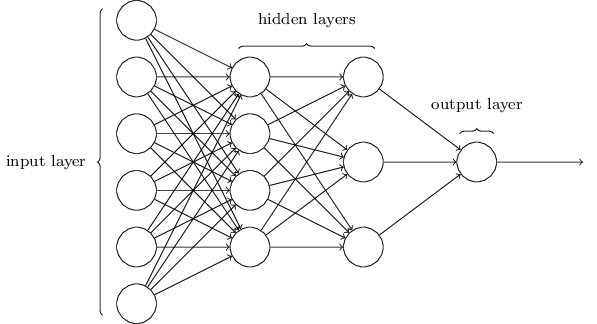
\includegraphics[scale=0.55]{figures/nnstructure.png}
 \caption{Neural Network structure}
 \label{nns}
 %\end{wrapfigure}
\end{figure}
These connections are mathematically described by weights, such as the input
of a neuron is determined by
\[
 y_i = \mathbf{w}_i \cdot \mathbf{x} + b_i = \sum_{j=1}^{q}w_{ij}x_j + b_i
\]
where $\mathbf{x}$ is the input values vector or the outcome of the
previous layer, $\mathbf{w}_i$ is instead the weight vector that corresponds
to the $i$-th neuron. A function $h$ is then applied to each of the $i$
neurons, it is called layer \textit{activation function} and it
yields as an output $\mathbf{z}=\{ z_i = h(y_i)\colon i = 1,\ldots,q\}$. This
process is being repeated through the network until the output layer is
reached.
There are some options for initializing weights
\begin{itemize}
 \item all initialized to a fixed value
 \item campionated from standard gaussian distribution
 \item campionated from uniform distribution
 \item other distributions
 \item etc.
\end{itemize}
it has been chosen to campionate them from a standard gaussian distribution.

The next step is understand how well the model predicts labels from data.
To achieve this we choose a \textit{loss function} that has the
characteristic to become smaller and smaller as the model learn, \eg~
perform better. Hence, the job is minimizing this function. In order to achieve
it several optimizing algorithms, or optimizers, exist.
The description of (some of these/the smoothest one: sgd) is given in
the next section.

Had obtained the neural network model, it is remarkable to note that there
is a theorem that states~\cite{theorem}
\begin{teorema}
 Feedforward networks are capable of arbitrarily accurate approximation
 to any real-valued continuous function over a compact set.
\end{teorema}

This is clearly excellent for us. Despite the fact that under certain
hypothesis almost every function can be represented by a neural network,
the maximum complexity achievable, however, depend on the choice of some of the
hyperparameters. Such as the number of layers, the number of neurons
for layer and the activation functions. A bad choice of these
hyper-parameters leads to a poor model that can not generalize well the problem
(underfitting) or a too complex model that does not fit well (overfitting).
On the other hand, the learning process itself must be
performed taking into account a series of issues that can lead to
underfitting or overfitting. Refer to~\cite{deeplearningbook} regarding
this (vast) topic.
\subsection{SGD}
The algorithm. A brief derivation. Some formulas.


\subsection{others..?}
Same.

\section{the physics of LHC}

The \textit{European Organization for Nuclear Research}, known as
\textit{CERN}, is a European research organization that operates the
largest particle physics laboratory in the world. \textit{CERN} is the
host of the \textit{Large Hadron Collider} (\textit{LHC}), the largest
particle accelerator in the world. Along its circumference four detectors
are arranged. \textit{CMS}, \textit{ATLAS} and \textit{LHCb} detect only
proton-proton collisions while \textit{ALICE} is used with collisions
between lead ions too. These four experiments carried on at \textit{LHC}
detect a great number of hadrons collisions per second and for each event
are record various forms of data. The large size, the variety and the high
rate of collisions production at \textit{LHC} are the reasons are named
\textit{big data} and these are one of the most suitable dataset for
testing efficiency of Neural Networks techniques. On the other hand,
employing more and more efficient machine learning algorithms to
\textit{LHC} datasets will let high energy physics community to extract
from data more information. This would reduce the waste of data.

\begin{figure}[htpb]
 \centering
 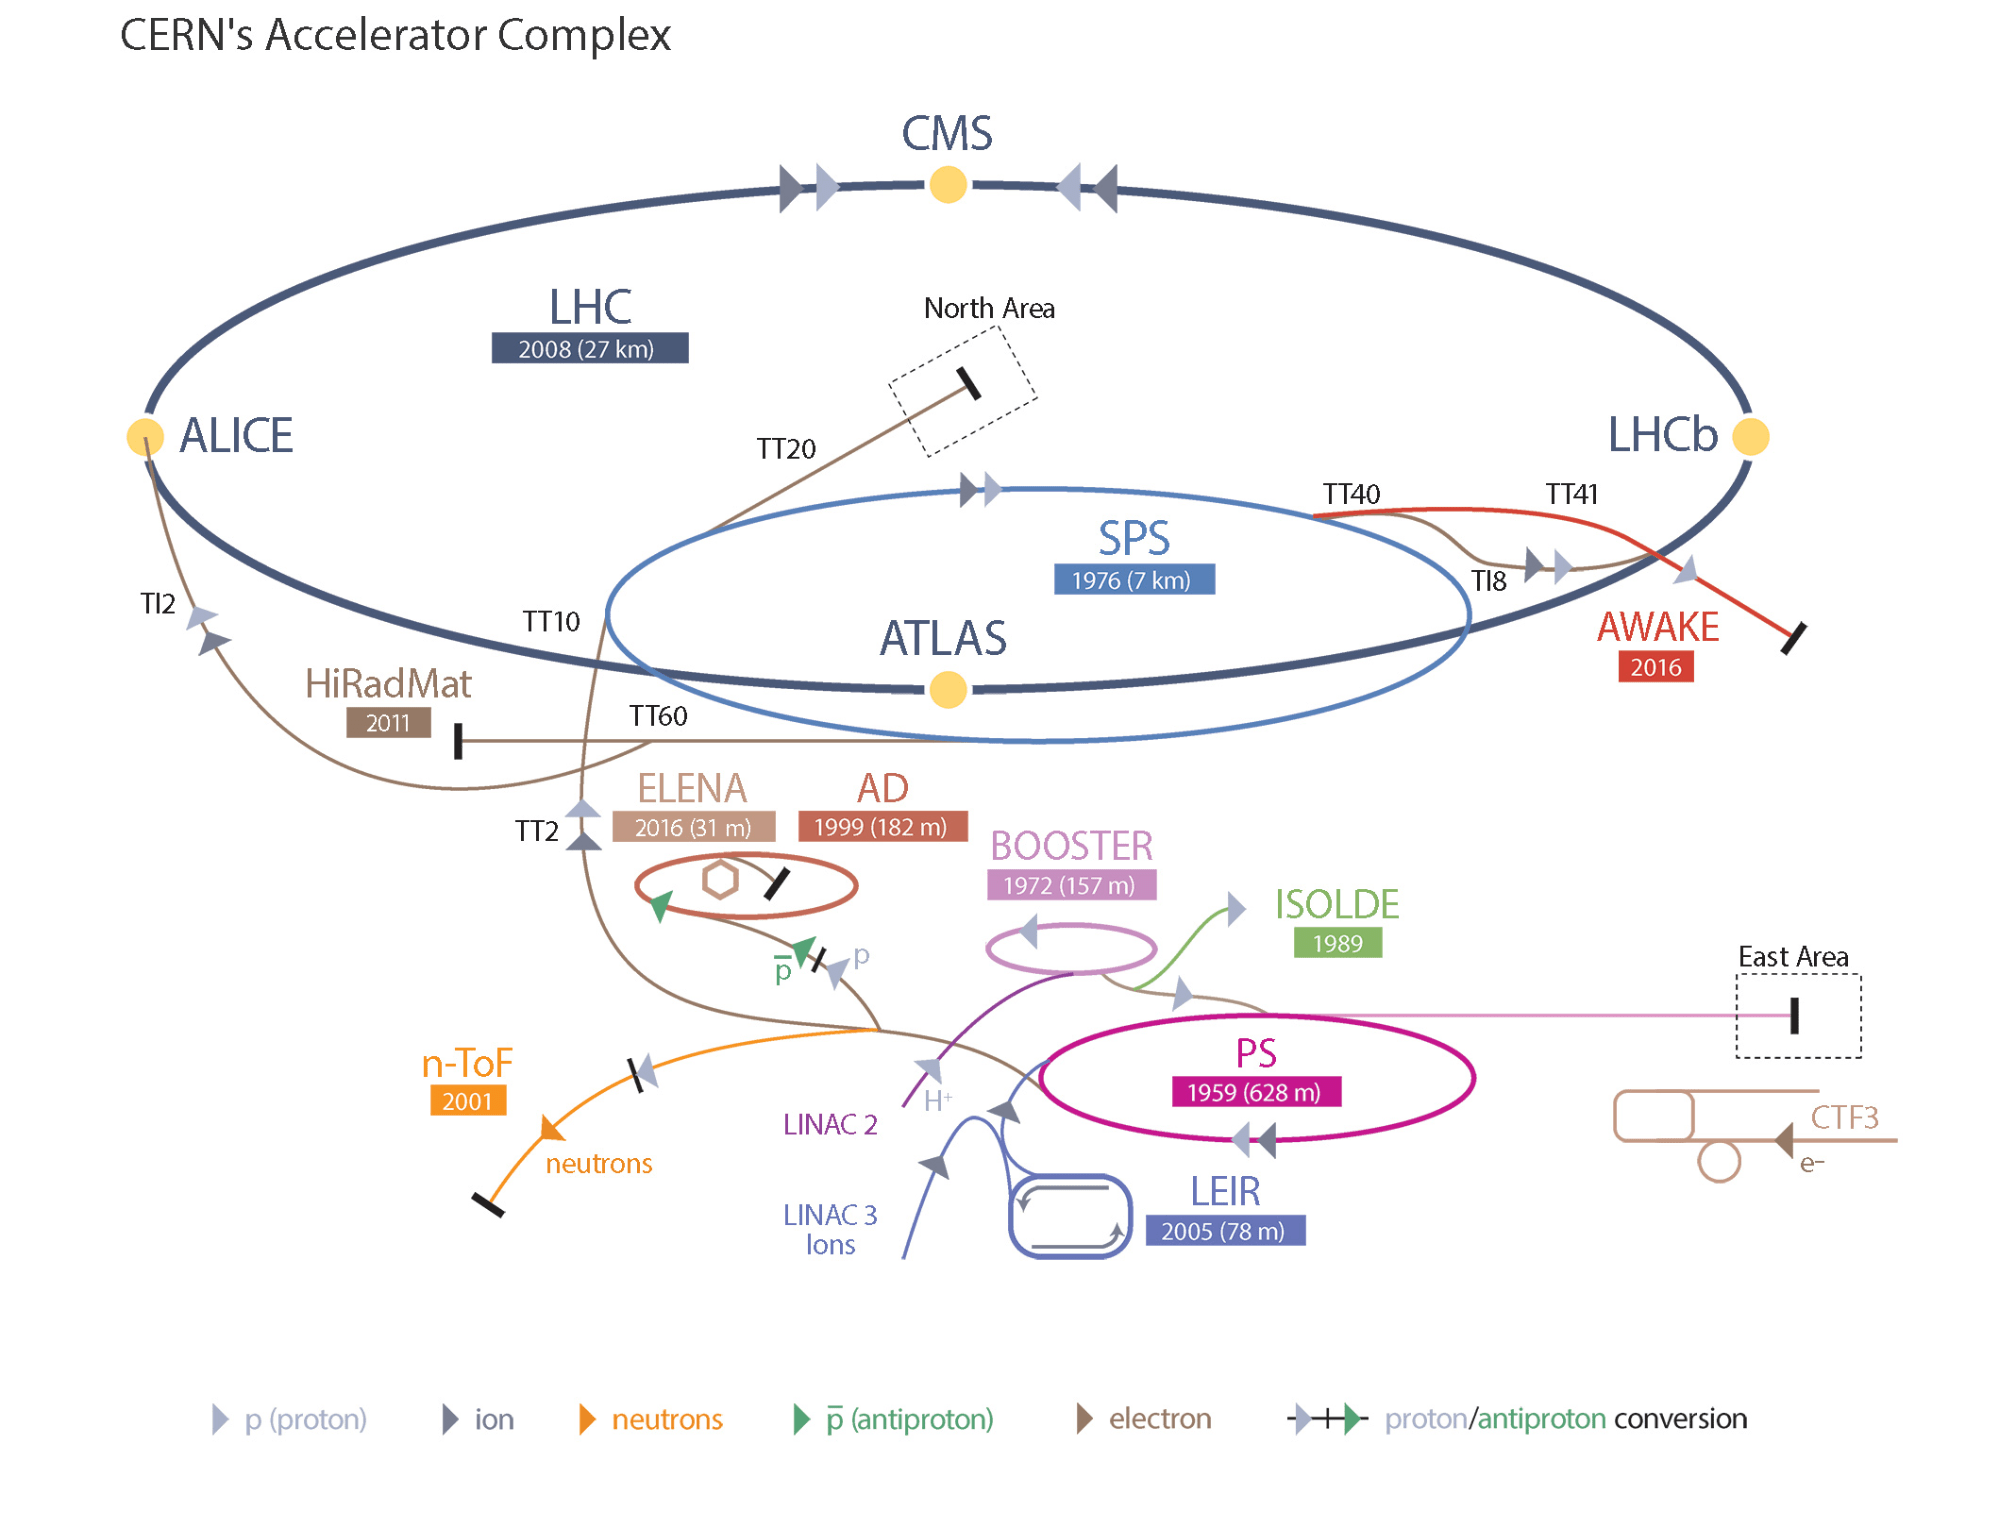
\includegraphics[scale=0.18]{figures/lhc2.png}
 \caption{\textit{LHC} complex}
 \label{}
\end{figure}

The \textit{LHC} accelerator itself consists of a $27$-kilometer ring of
superconducting magnets with a number of accelerating cavities to make
beams focused in order to maximize the cross section. Also for curve the
trajectory and increase the energy of the particles circulating inside its
rings. The preparatory phase pf acceleration begin at the Linac 2 where the
protons from hydrogen are accelerated to $50$ MeV. The beam is then get
injected into the Proton Synchrotron Booster (PSB) where the proton bunches
are formed and accelerated further to $1.4$ GeV. The next accelerator is
called the Proton Synchrotron (PS) which forms the final shape of the beam
bunches and kicks the beam up to $25$ GeV. The particles are later sent to
the Super Proton Synchrotron (SPS) where they are accelerated to $450$ Gev,
from which they are injected into two pipes of the \textit{LHC}. This is
where the beams go in opposite directions to be collided at the
experimental sites with up to a center-of-mass energy of $\sqrt{s}=14$ TeV.

Taking the CMS detector as an example it is formed by a series of cylindrical
sub-detectors able to detect different interactions. This for the purpose
of study many aspects of the high energy interactions between protons, from
the Standard model parameters to the New Physics theories and their
associated particles. Different technologies are used to observe different
features of the particles going across them. The closest one is a vertex
detector of silicon pixels and strips used to track charged particles near
to the point of interaction. Then there is the charged particle tracking
chamber which distinguishes positive and negative charges measuring the
curvature of the particles in a magnetic field. Next layer consists in two
calorimeters: one absorbing the electromagnetic-showers and the other the
hadronic-showers. Finally, the muon chambers which absorb the heaviest
particles called muons. All these components together are able to absorb
all the energy issued by the collision except that carried out by
neutrinos. From the pieces of information collected by each layer of the
detector, high energy physicists are able to go back to the nature of the
particles produced by the collision and study the laws which regulate these
processes.

\begin{figure}[H]
 \centering
 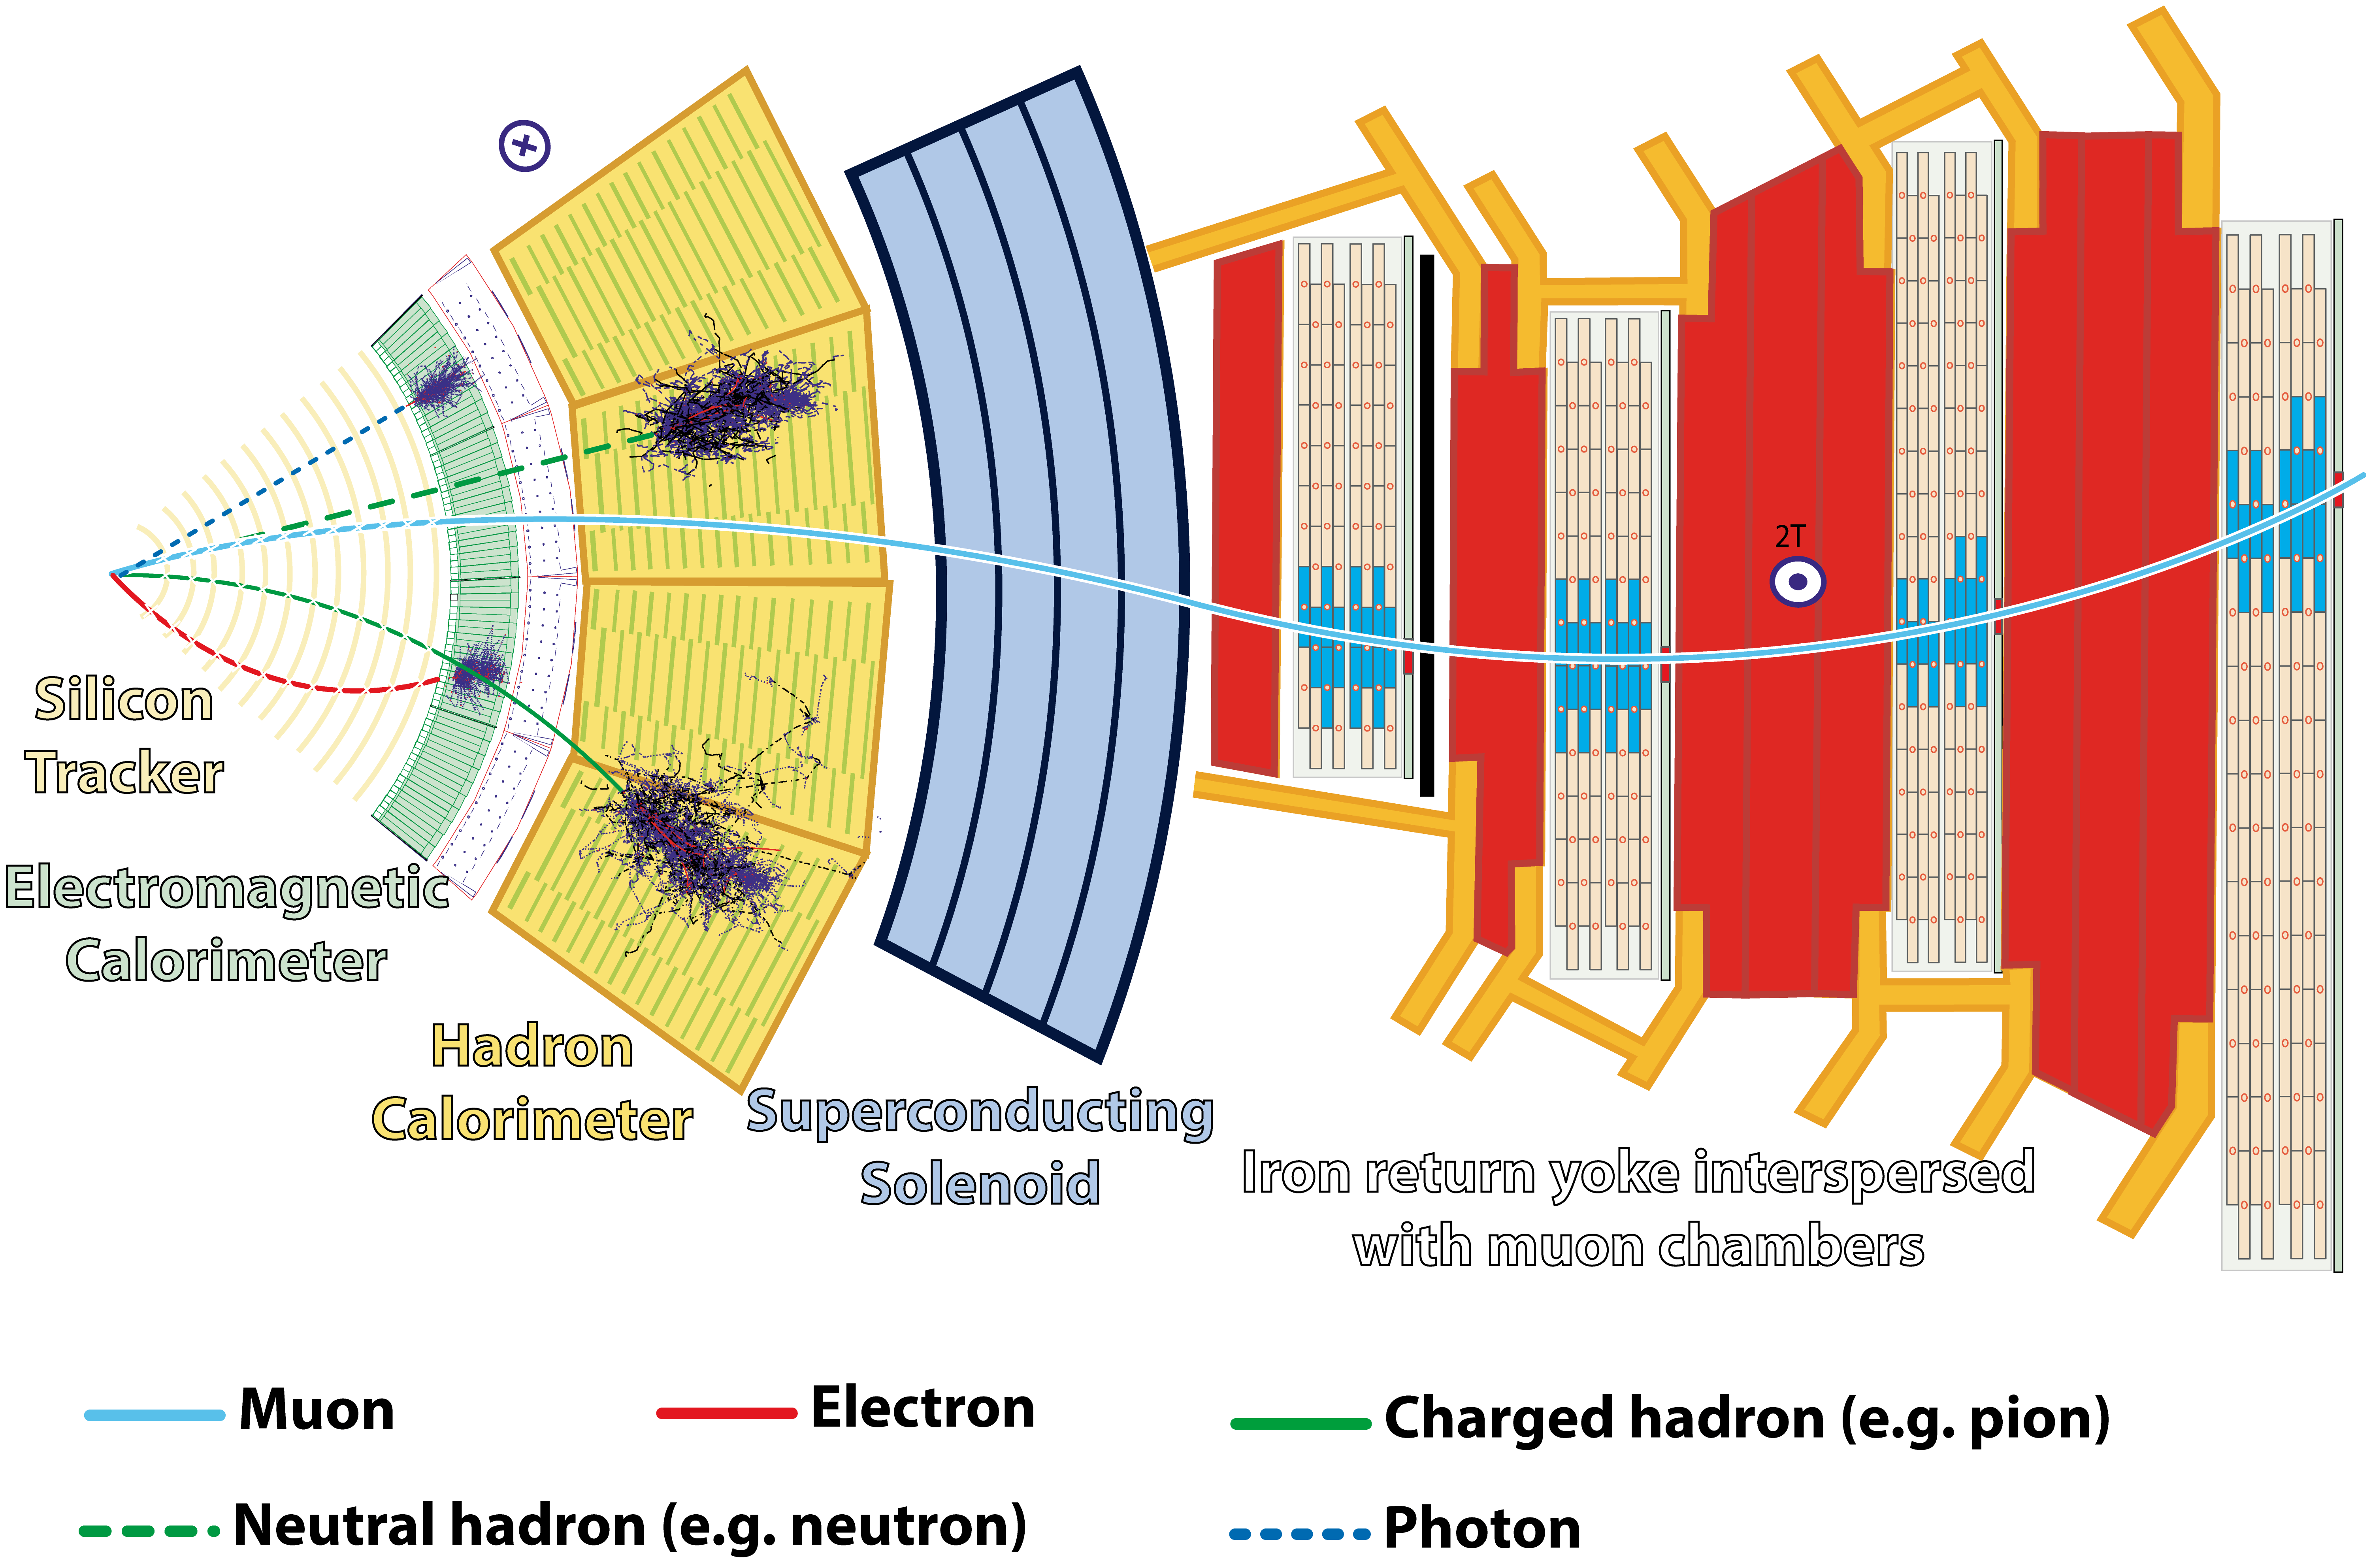
\includegraphics[scale=0.05]{figures/CMSslice.png}
 \caption{A transverse section of the CMS detector}
 \label{}
\end{figure}

\section{The benchmark dataset HIGGS}\label{data}%\footnote{The features
% distribution are in the Appendix}
The dataset subject of this work involves a signal process where new Higgs
bosons are produced and a background process with identical decay products
but distinct kinematic features.
The signal process is the fusion of two gluons into a heavy
electrically-neutral Higgs boson ($gg \rightarrow H^0$), which decays
to a heavy electrically-charged Higgs boson ($H^\pm$) and a $W$ boson.
The $H^\pm$ subsequently decays to a second $W$ boson and in a light Higgs
boson, $h^0$. The light Higgs boson then decays predominantly to a pair of
bottom quarks. The entire process is then:
\begin{equation}
 gg \rightarrow H^0 \rightarrow W^\mp H^\pm \rightarrow W^\mp W^\pm h^0
 \rightarrow W^\mp W^\pm b \bar{b}
\end{equation}
which leads to $W^\mp W^\pm b \bar{b}$. The background process, which
mimics $W^\mp W^\pm b \bar{b}$ without the Higgs boson intermediate state
is the production of a pair of top quarks, each of which decays to $Wb$
(see figure 1.):
\begin{equation}
 gg \rightarrow g \rightarrow t\bar{t} \rightarrow W^\mp W^\pm b \bar{b}
\end{equation}

\begin{figure}[htpb]
 \centering
 \subfloat[][]{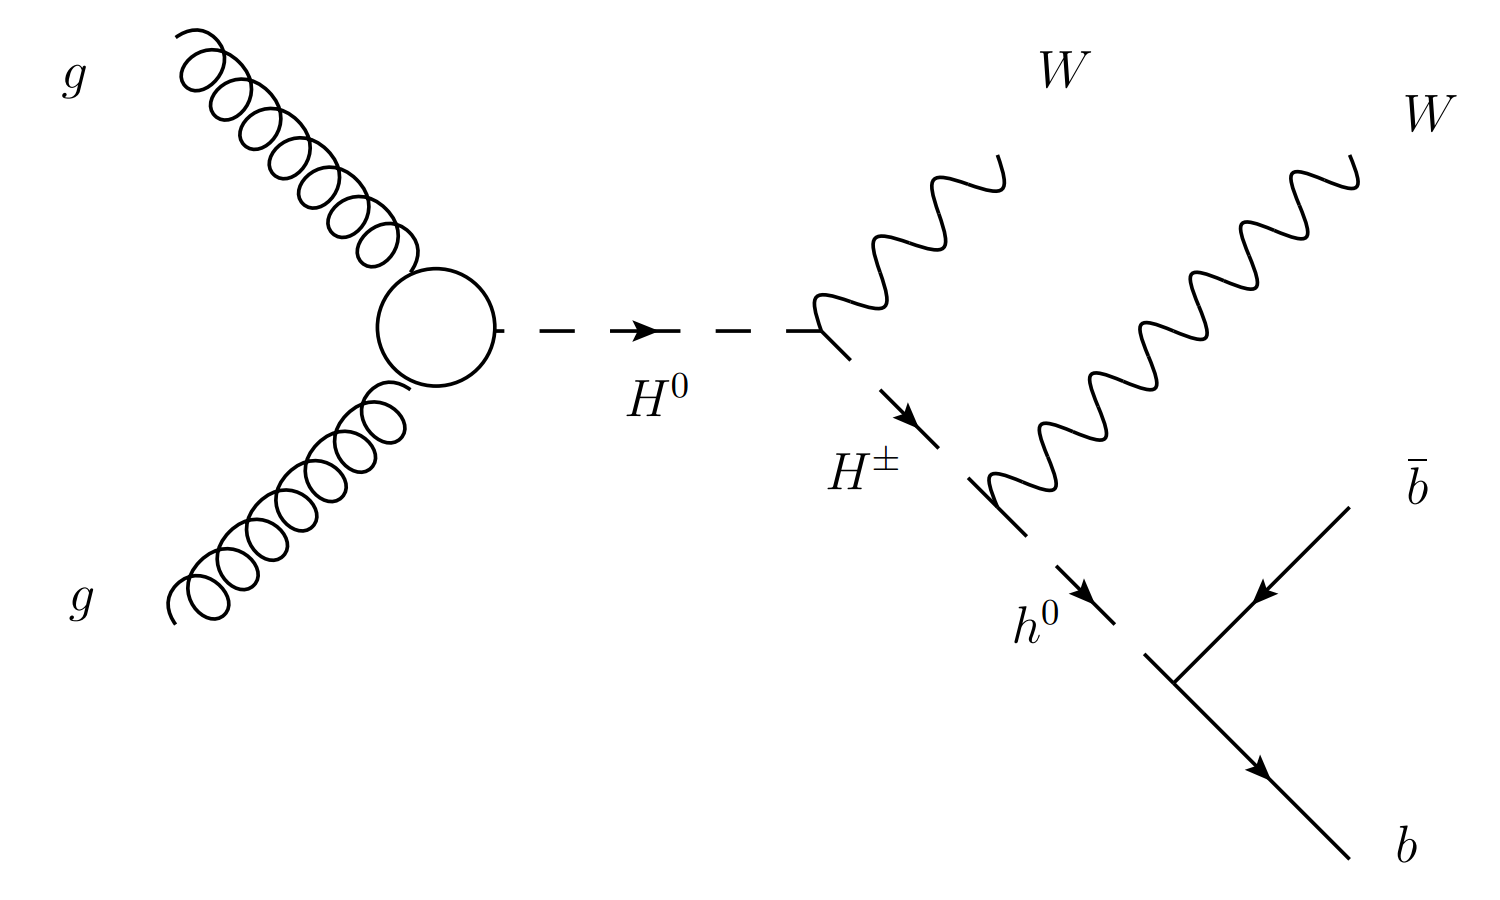
\includegraphics[width=.45\textwidth]{figures/decs.png}} \quad
 \subfloat[][]{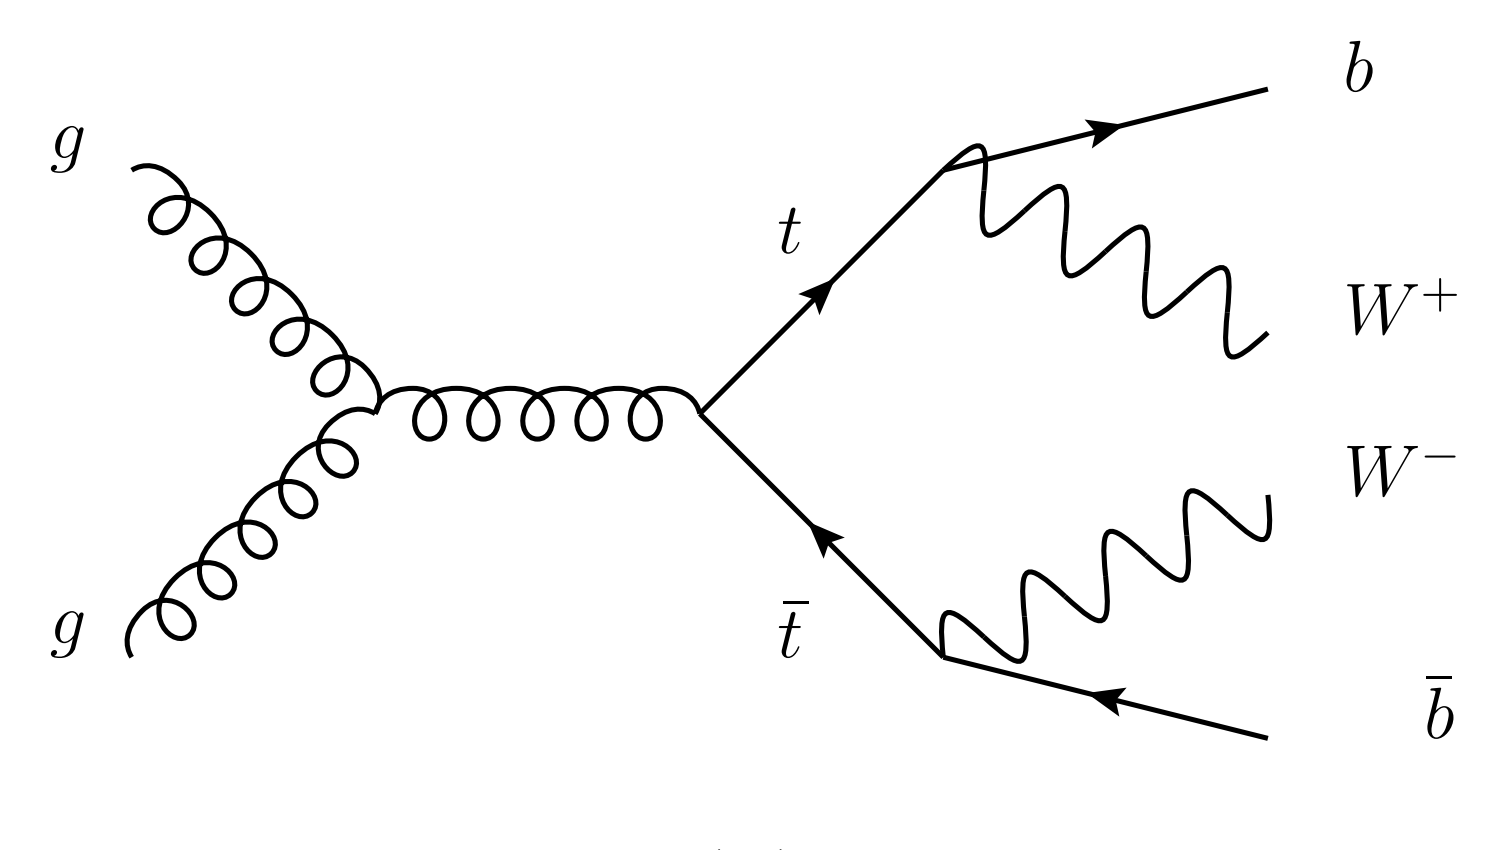
\includegraphics[width=.45\textwidth]{figures/decb.png}} \\
 \caption{(a) Diagram describing the signal process involving new exotic
  Higgs bosons $H^0$ and $H^\pm$. (b) Diagram describing the background
  process involving top-quarks ($t$). In both cases, the resulting
  particles are two $W$ bosons and two $b$-quarks.}
 \label{graphs}
\end{figure}

accordingly, to~\cite{paper} the events are simulated assuming $8$ TeV
collisions of protons at LHC. For the benchmark case here, $m_{h^0}=125$
GeV, $m_{H^0}=425$ GeV and $m_{H^\pm}=325$ GeV has been assumed.
In order to simulate events for this dataset the semi-leptonic decay mode has
been chosen, which is one $W$ boson decaying to a lepton and a
neutrino($l\nu$) and the other $W$ boson in a pair of jets (which
correspond to a couple of up-type and down-type quarks). Thus, the
final products of our decays are $l\nu b j j  b$.
In \cite{paper} has been considered events which satisfy (and we do
accordingly):
\begin{itemize}
 \item exactly one electron or muon, with $p_T > 20$ GeV and
       $\vert \eta \lvert < 2.5$
 \item at least four jets, each with $p_T > 20$ GeV and
       $\vert \eta \lvert < 2.5$
 \item $b$-tags on at least two of the jets, indicating that they are
       likely due to $b$-quarks rather than gluons or lighter quarks
\end{itemize}

where $p_T$ is the momentum transverse to the beam direction and
(referred to a polar coordinate system) the polar angle $\theta$
is substituted by
\[
 \eta = -\ln{\tg{\frac{\theta}{2}}}
\]
there is then the azimuthal angle $\phi$.
The above requirements are then summed up by 21 low-level features:
\begin{itemize}
 \item $4$ jets, each of them described through $4$ variables: $p_T$,
       $\eta$, $\phi$ and the $b$-tag.
 \item $1$ lepton described through 3 variables: $p_T$, $\eta$, $\phi$
 \item $1$ neutrino indirectly described by: missing energy magnitude and
       missing energy $\phi$
\end{itemize}

Theoretical considerations allow constructing new high level features
which better highlight the differences between these two processes.
The features are the invariant masses of the metastable particles.
In particular, for signal processes the following resonant decays have
been theorized and the related invariant masses have been computed:
\begin{itemize}
 \item $W \rightarrow l \nu$: the invariant mass $m_{l\nu}$ should show
       in the known mass of the $W$ boson $m_W$
 \item $W \rightarrow jj$: the invariant mass $m_{jj}$ should show a peak
       at the known mass of the $W$ boson $m_W$
 \item $h^0 \rightarrow b\bar{b}$: $m_{b\bar{b}}$ should show a peak at
       $m_{h^0}$
 \item $H^\pm \rightarrow W^\pm h^0$: $m_{Wbb}$ should show a peak at
       $m_{H^\pm}$
 \item $H^0 \rightarrow WH^\pm$: $m_{WWb\bar{b}}$ should show a peak at
       $m_{H^0}$
\end{itemize}
there represent $5$ high-level features. On the other hand,
regarding $t\bar{t}$ background, it is expected that:
\begin{itemize}
 \item $W \rightarrow l \nu$ shows a peak in $m_{l\nu}$ at $m_W$
 \item $W \rightarrow jj$ shows a peak in $m_{jj}$ at $m_W$
 \item $t \rightarrow Wb$ shows a peak in $m_{jl\nu}$ and $m_{jb\bar{b}}$ at
       $m_t$
\end{itemize}
thus two more invariant masses $m_{l\nu b}$ and $m_{jjb}$ have been
computed. In total there are 7 high-level features. Before being passed to
the neural networks the dataset had been standardized removing mean and
standard deviation from features. The just described sample with 11 million
events is available in the UCI machine learning
repository.\footnote{https://archive.ics.uci.edu/ml/datasets/HIGGS}


\section{The setup (bigdl?)}

The used hardware is composed by a six nodes (computers) cluster hosted by
Cloudveneto\footnote{https://cloudveneto.ict.unipd.it/} and a GPU machine
under the same domain. In a cluster, one node is called cluster manager or
master, while the others workers or slaves.
In this case, the master is a computer with $2$ cores and
$\SI{4}{\giga\byte}$ of RAM while the $5$ nodes are computers with $8$
cores and $\SI{16}{\giga\byte}$ of RAM, for a total of $40$ cores and
$\SI{80}{\giga\byte}$ of RAM for the slaves.
The master role is to dispatch individual small tasks to the slaves that
send back the processed results. This paradigm is carried out by Apache
Spark\cite{spark} which is a \textit{unified analytics engine for large-scale
 data processing}\footnote{https://spark.apache.org/}.
Spark applications run as independent sets of processes coordinated by the
\lstinline{SparkContext}
object in the main program (\textit{driver program}).
Specifically, to run on a cluster, the SparkContext connect
to a \textit{cluster manager} which allocate resources across applications.
Once connected, Spark acquires \textit{executors} on nodes in the cluster,
which are the processes that run computations and store data to process.
Next, it sends the application code to the executors. Finally, SparkContext
sends \textit{tasks} to the executors to run.
\begin{figure}[htpb]
 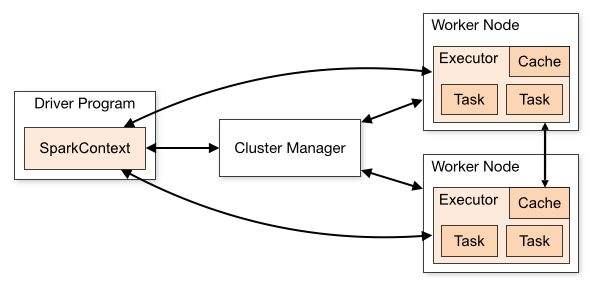
\includegraphics[scale=0.55]{figures/cluster-overview.png}
 \caption{The Spark architecture}
 \label{}
\end{figure}

The driver program has been written in Python\footnote{https://www.python.org/}
which is a high level programming language widely used nowadays for data
science topics. In the program, through Spark application program interface
(API), instructions are sent to workers. Spark use as backend Java, meaning
that the execution of the Spark code is committed to a Java interpreter which
is a lower level programming language. This is a common programming paradigm,
the code is written in a higher level language while the actual execution is
performed by a lower one. Python itself is written in \CC~which is one of the
oldest and still very used low level programming language.

While the framework used is Spark, the utilized library for implementing the
distributed Deep Neural Network models is BigDL~\cite{bigdl} from Intel
Corporation. Instead, for the standalone and the GPU version has been used
Keras~\cite{keras} with Tensoflow~\cite{tensorflow} backend.

The work done in~\cite{gaia} and~\cite{paper} has been used for fix some
hyperparameters:
\begin{itemize}
 \item Number of layers: $3$
 \item Neuron for layer: $300$
 \item Dropout: $0$
 \item Layer activation function: \textit{tanh}
 \item Output activation function: \textit{sigmoid}
 \item Learning Rate: Default value of the optimizer
\end{itemize}

For what concern the hidden layers activation function the
$tanh$ function has been chosen. Instead, for the output neuron a sigmoid
has been taken.
\begin{figure}[h]
 \begin{minipage}{.5\textwidth}
  \begin{equation*}
   \tanh(x) = \frac{\me^x-\me^{-x}}{\me^x+\me^{-x}}
  \end{equation*}
  \begin{equation*}
   \text{sig}(x)=\frac{1}{1+\me^{-x}}
  \end{equation*}
 \end{minipage}%
 \begin{minipage}{.5\textwidth}
  \centering
  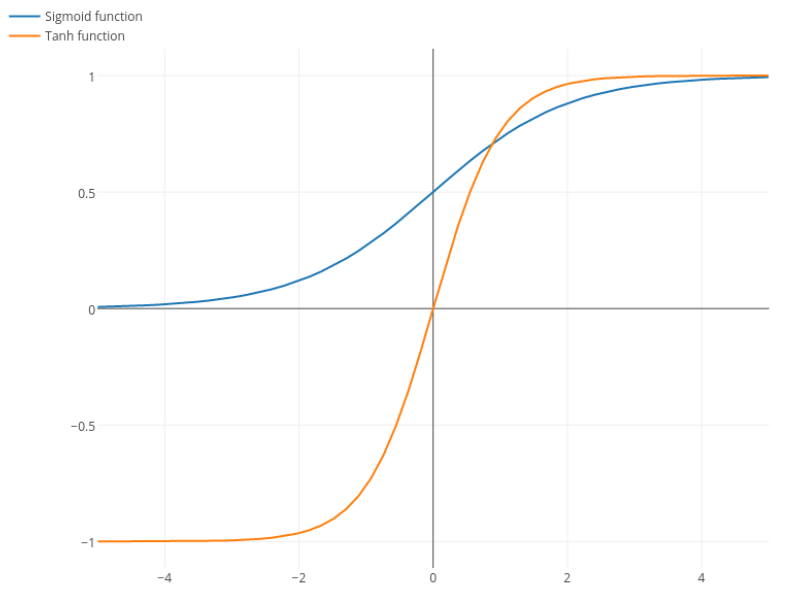
\includegraphics[scale=0.3]{figures/SeT.png}
 \end{minipage}
 \caption{tanh and sigmoid functions comparison}
\end{figure}

The sigmoid function has the property of returning an output in the interval
$\left(0,1\right)$ it can be seen as the confidence the network has
regarding the $0$ or the $1$ classification. It means that the closer to $1$
is the output the more confident the network is about the event
classification as a signal, vice versa a result near $0$ means a background
event. It is a very common choice for an output function for a Machine
Learning classifier.

% chktex-file 46
%!TeX spellcheck = en-US,it-IT
\chapter{Neural Networks performance analysis}

Different variety of Neural Networks exist. The used one in this thesis,
and the description that was given, is about Feedforward Networks.
Depending on the number of hidden layers they are called Shallow Neural
Networks ($1$) and Deep Neural Networks ($>1$).
\begin{figure}[h]
 %\begin{wrapfigure}{r}{0.33\textwidth} %this figure will be at the right
 \centering
 %    \includegraphics[width=0.25\textwidth]{mesh}
 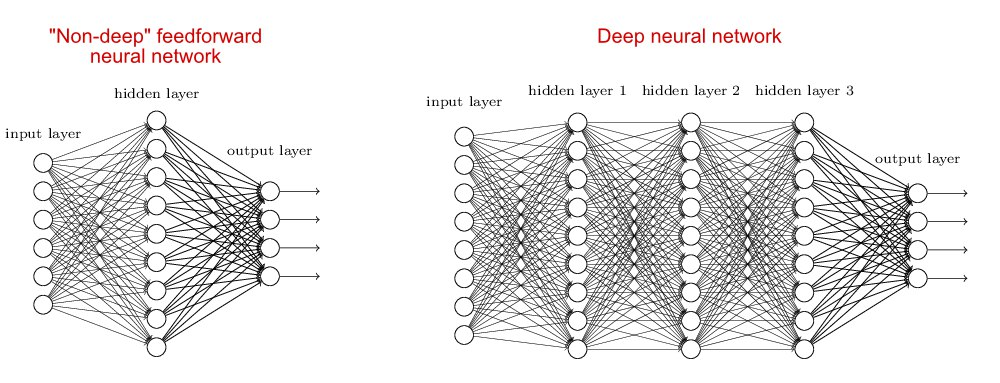
\includegraphics[scale=0.4]{figures/svsd.jpeg}
 %\end{wrapfigure}
\end{figure}

The main focus of~\cite{paper} and~\cite{gaia} is to demonstrate that
performance of the two kinds is comparable when using high level features
for the shallow one and low level features for the deep one. To achieve this
it is need a \textit{metric}, a measure of how well the classificator is
performing. Evaluating the metrics over the training, validation and test sets
is the primary technique for point out how the training process is going.
Therefore, is crucial to use the most significant ones.

The default metric provided by Keras~\cite{keras} is the binary accuracy.
Given an event if the output is greater than $0.5$ then it is classified
as signal, background otherwise. The right label is then compared and the
prediction correctness is determined. Done it for the entire considered
subset and found the right prediction percentage  the (binary) accuracy
is obtained.
Another metric widely used in Machine Learning is the result loss function
considered as a mean over a subset of events. This is the number that the
optimizer itself is trying to minimize so is a direct performing rate.
Despite this, it is significant in the training process only. It can not be
used in the final classifier rating not having a statistical meaning.
\begin{figure}[h]
 \centering
 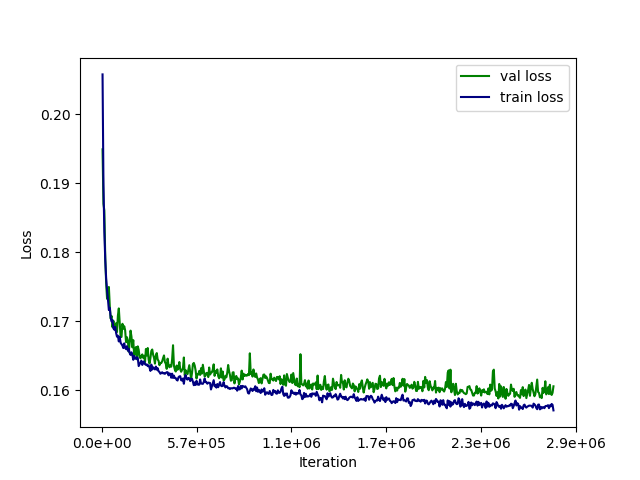
\includegraphics[scale=0.4]{figures/loss_tv.png}
 \caption{loss function during training}
\end{figure}

A more statistically significant approach is to find the \textit{AUC}
score, \ie~the \textit{Area Under the ROC Curve}, by drawing and
integrating the \textit{ROC Curve} that stands for \textit{Receiver
 Operating Characteristic}. Drawing the ROC curve is a graphical method to
observe binary classifiers efficiency. It is done by plotting percentage
successfully signal prediction (signal efficiency) versus the percentage
successfully background discovery \#(classification?) (background rejection).
The various points of the graph are obtained by varying the threshold in
the interval $\left[0,1\right]$ beyond which the Neural Network output it
considered signal, note that the binary accuracy is essentially the
ROC point which threshold is $0.5$.
\begin{figure}[h]
 \begin{minipage}{.5\textwidth}
  \centering
  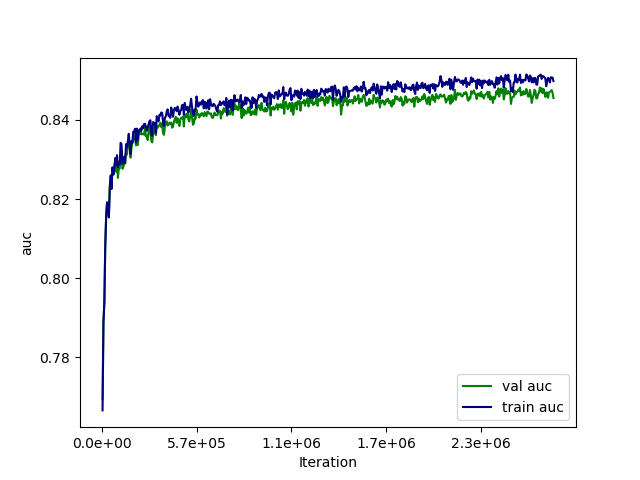
\includegraphics[scale=0.4]{figures/auc_tv.png}
  \caption{auc score during training}
 \end{minipage}\qquad%
 \begin{minipage}{.5\textwidth}
  \centering
  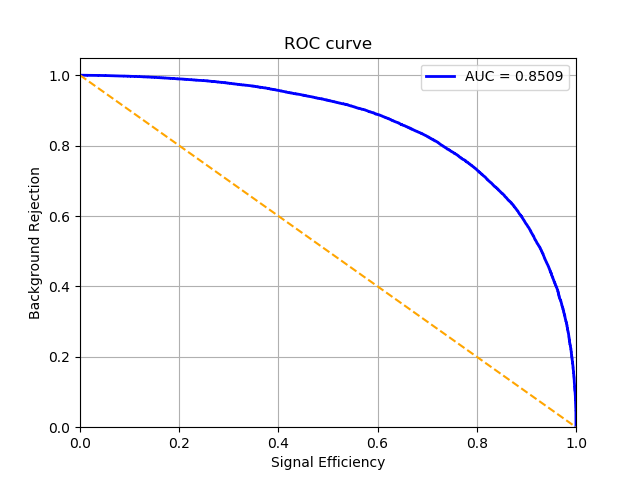
\includegraphics[scale=0.4]{figures/test_auc.png}
  \caption{test set auc score}
 \end{minipage}
\end{figure}

One more quantity that highlights the model behavior is called
\textit{Figure Of Merit} (\textit{FOM}). It is defined as
$FOM = \frac{S}{\sqrt{B}}$ where $S$ is the right classified signal events
total number and $B$ is right classified background events total number.
The term $\sqrt{B}$ represents the error on the number of background events
assuming they follow a Poisson distribution. More precisely, to state
whenever signal events $S$ are actually a resonance or only statistical
fluctuations, the effective error should take into account also the error on
the number of signal events, that is $\sqrt{S}$, as signal follow
poissonian distribution too. So the correct expression for the error would
be $\sigma = \sqrt{B + S}$. Nonetheless since $S \ll B$ the error can be
approximated as $\sigma \approx \sqrt{B}$.
\begin{figure}[h]
 \centering
 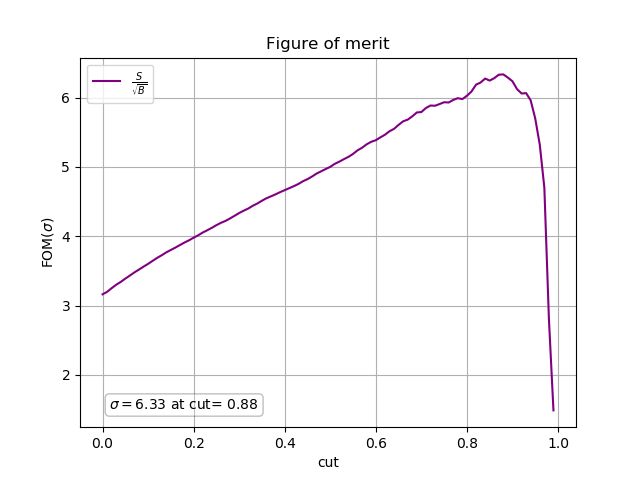
\includegraphics[scale=0.4]{figures/fom.png}
 \caption{Figure of merit of the test set}
\end{figure}

The data were simulated as described in Section~\ref{data} and they were
built such that signal and background would have the same probability.
The consequence is that the number of signals predicted events should be
quite the same of background predicted. In data collected by experiments, a
signal of new physics is usually a rare phenomenon which competes with
lots of standard processes included in background. Thus, the real cross
section of signal events may be so small that it may be confused with
background. $FOM$ computation allows finding the optimal cut point to
put in evidence the presence of signals. In fact, maximize this quantity
considered as a  function of the classifier acceptance threshold means
maximizing signal and background distribution over the phase space
expected by the theoretical model. A good cut point choice allows
physicists to determine whenever a difference in experimental
distributions can be identified as a new signal or not.

The last performance indicator that has been considered is the histogram
of the predicted events over the possible model outcomes. The network
discriminates well if the predicted signal distribution present a peak
towards $1$ and the predicted background distribution towards $0$.
\begin{figure}[h]
 \centering
 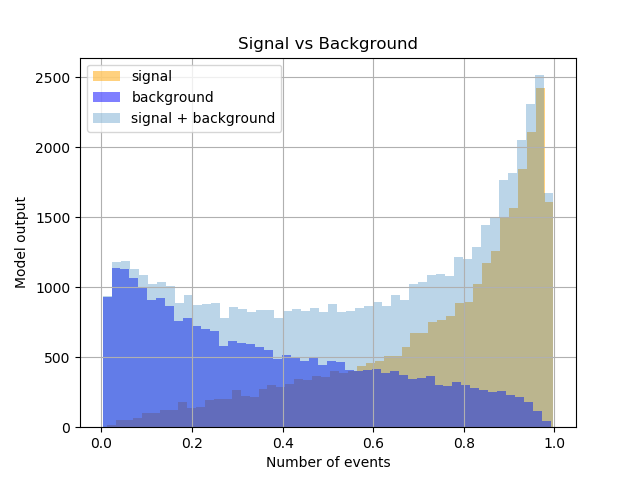
\includegraphics[scale=0.4]{figures/svb.png}
 \caption{Signal versus background in test set}
\end{figure}

\section{Shallow and deep Neural Networks performance}

In~\cite{gaia} some experiments have been done varying the number of layers,
neurons for layer and using various regularization techniques. The most
interesting result obtained is that the Deep Neural Networks trained and
tested with low level features perform the same (or better) than the Shallow
Neural Networks with high level features, which is excellent given the not
negligible work needed to develop high level features. The same results are
also found in~\cite{paper}.
\begin{figure}
 \centering
 \subfloat[][SN performance in~\cite{paper}]{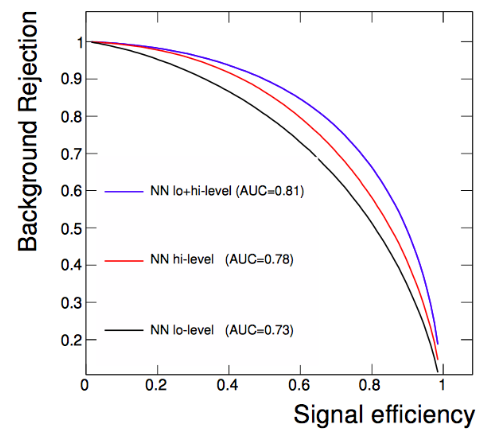
\includegraphics[width=.45\textwidth]{figures/SNp.png}} \quad
 \subfloat[][DN performance in~\cite{paper}]{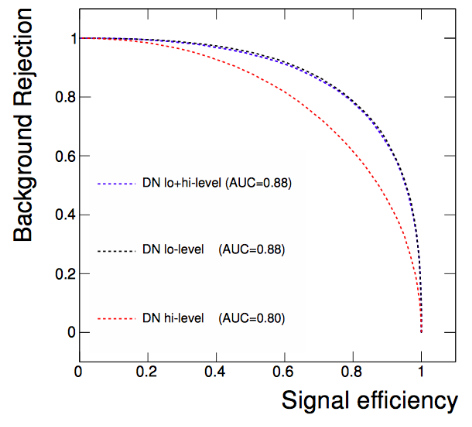
\includegraphics[width=.45\textwidth]{figures/DNp.png}} \\
 \subfloat[][SN performance in~\cite{gaia}]{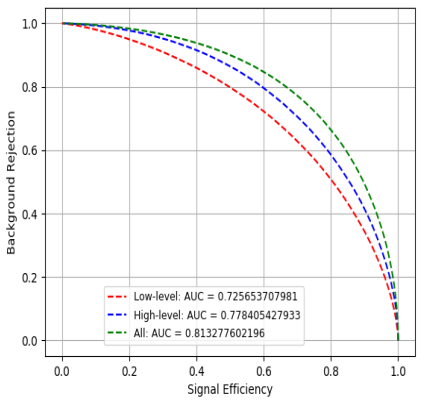
\includegraphics[width=.45\textwidth]{figures/SNg.png}} \quad
 \subfloat[][DN performance in~\cite{gaia}]{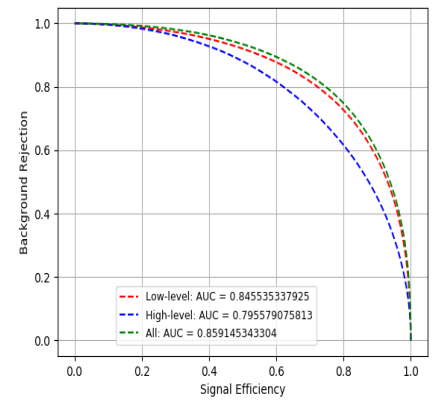
\includegraphics[width=.45\textwidth]{figures/DNg.png}} \\
 \caption{}
 \label{graphs}
\end{figure}
In Fig.~\ref{graphs} and in Tab.~\ref{table} are shown a comparison of the
performance with shallow neural networks (SNN) and deep neural networks
(DNN) in~\cite{paper} and~\cite{gaia} for three sets of input of features:
low level features, high level features and the complete set of features.
As can be seen, a shallow NN trained using only the low level features
performs significantly worse than one trained with only the high level
features. This is a well-known problem with shallow learning methods, and
motivates the calculation of high level features. Methods trained with only
the high level features, however, have a weaker performance than those
trained with the full set of features, which suggests that despite the
insight represented by the high level features, they do not capture all
the information contained in the low level features. The deep learning
techniques show close performance using the low level features
and the complete features, suggesting that they are automatically
discovering the insight contained in the high level features. The slightly
different performance in~\cite{paper} and~\cite{gaia} are explainable due
to the fact in~\cite{gaia} the algorithms can handle the training for
about $40$-$60$ epochs before overfitting, instead~\cite{paper} are able
to train for $200$-$1000$ which is a great difference. Even if the
quantitative results differ, the qualitative ones are the same.
\begin{table}
 \centering
 \subfloat[][AUC and discovery significance in~\cite{paper}]{
  \begin{tabular}{lccc}
   \toprule
   Technique                 & Low level   & High level  & Complete    \\
   \midrule
   $\text{SNN}_{\text{auc}}$ & $0.733$     & $0.777$     & $0.816$     \\
   $\text{DNN}_{\text{auc}}$ & $0.880$     & $0.800$     & $0.885$     \\
   $\text{SNN}_{\text{DS}}$  & $2.5\sigma$ & $3.1\sigma$ & $3.7\sigma$ \\
   $\text{DNN}_{\text{DS}}$  & $4.9\sigma$ & $3.6\sigma$ & $5.0\sigma$ \\
   \bottomrule
  \end{tabular}
 } \\
 \subfloat[][AUC and discovery significance in~\cite{gaia}]{
  \begin{tabular}{lccc}
   \toprule
   Technique                 & Low level    & High level   & Complete     \\
   \midrule
   $\text{SNN}_{\text{auc}}$ & $0.675$      & $0.763$      & $0.812$      \\
   $\text{DNN}_{\text{auc}}$ & $0.846$      & $0.796$      & $0.858$      \\
   $\text{SNN}_{\text{DS}}$  & $3.34\sigma$ & $3.69\sigma$ & $4.11\sigma$ \\
   $\text{DNN}_{\text{DS}}$  & $4.44\sigma$ & $3.85\sigma$ & $4.66\sigma$ \\
   \bottomrule
  \end{tabular}
 }
 \caption{}
 \label{table}
\end{table}

To understand if the obtained results can help to discriminate new signals
assumption was made that for $100$ signals events were $1000$ background
events as can be seen in Fig.\ref{res}. In order to simulate the physical
reality prediction histograms were re-normalized. The Tab.\ref{table} show
then that the discovery significance, which is a standard metric in
high-energy physics, can significantly improve even with small increases in
AUC.

\begin{figure}[hb]
 \centering
 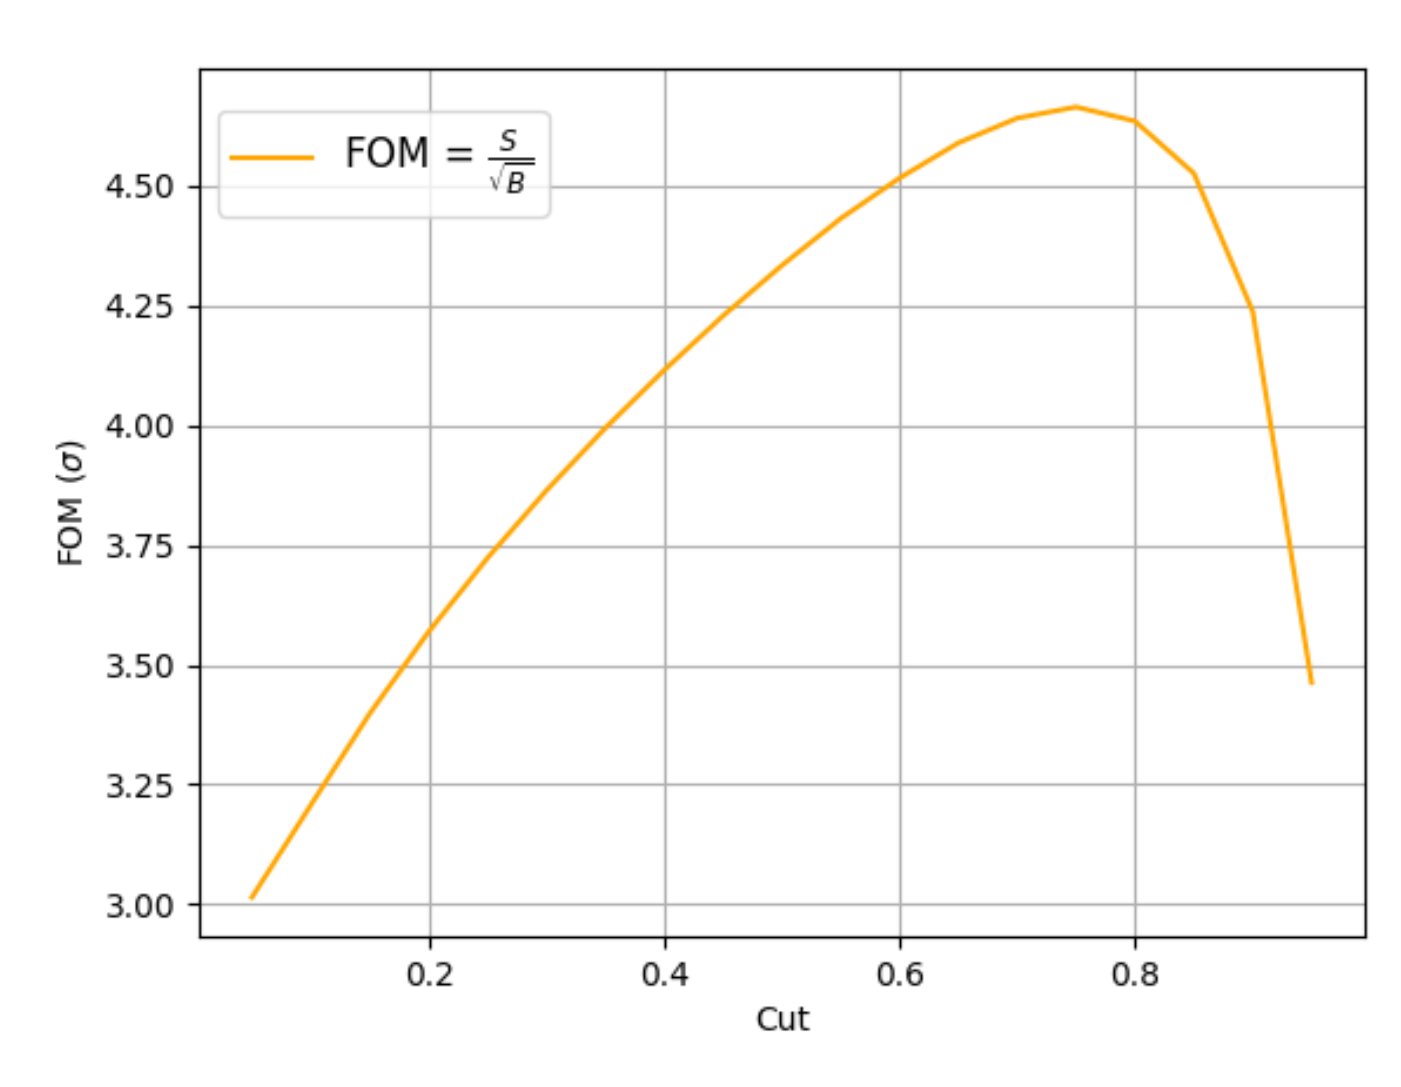
\includegraphics[width=.45\textwidth]{figures/fomr.png}
 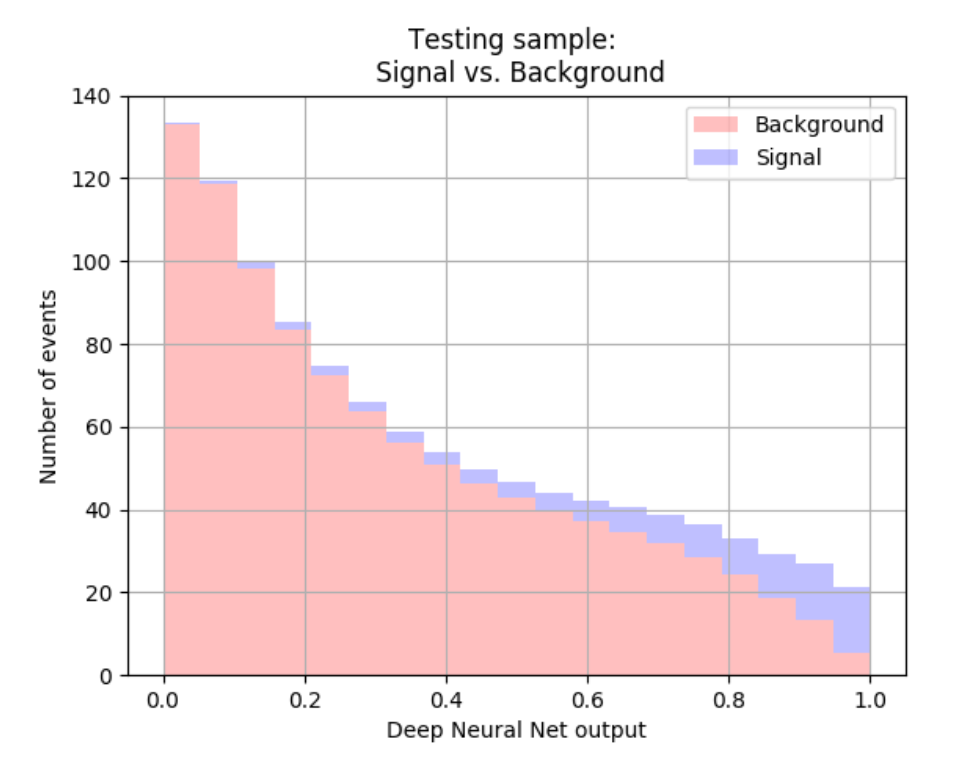
\includegraphics[width=.45\textwidth]{figures/svdbr.png}
 \caption{Figure of merit obtained after normalization in~\cite{gaia}}
 \label{res}
\end{figure}

%\ctparttext{}
\part{Results}\label{pt:results}
% chktex-file 46
%!TeX spellcheck = en-US,it-IT

\chapter{Cluster scalability}
In the thesis early stages, experiments have been done with the Distributed
Keras framework~\cite{distkeras} developed at CERN
but BigDL seemed more promising so we continued with this library.
Initially training was performed with a cluster formed of an $8$ cores master node and
$\SI{16}{\giga\byte}$ (\textit{xlarge}) and $5$ slaves with $2$ cores each
and $\SI{4}{\giga\byte}$ (\textit{medium}). Then it became clear
that, for the task, it was better an architecture with a \textit{medium} master and $5$
\textit{xlarge} slaves due to the fact that all the heavy lift is performed by workers.
On the GPU architecture side we had available an \textit{Nvidia Titan
 Xp}\footnote{https://www.nvidia.com/en-us/titan/titan-xp/} and an \textit{Nvidia RTX 2080
 FE}\footnote{https://www.nvidia.com/en-us/geforce/graphics-cards/rtx-2080/} graphics
cards.

We tested our model with several optimizers implemented by BigDL and Keras libraries.
The standard optimizer SGD, Adam\cite{Adam}, Adamax\cite{Adam}, Adadelta\cite{Adadelta}
and Adagrad\cite{Adagrad}. Cluster performance is evaluated between different numbers of
nodes and available GPUs. Results are shown in Fig.~\ref{1} and Fig.~\ref{2}.
\begin{figure}[H]
 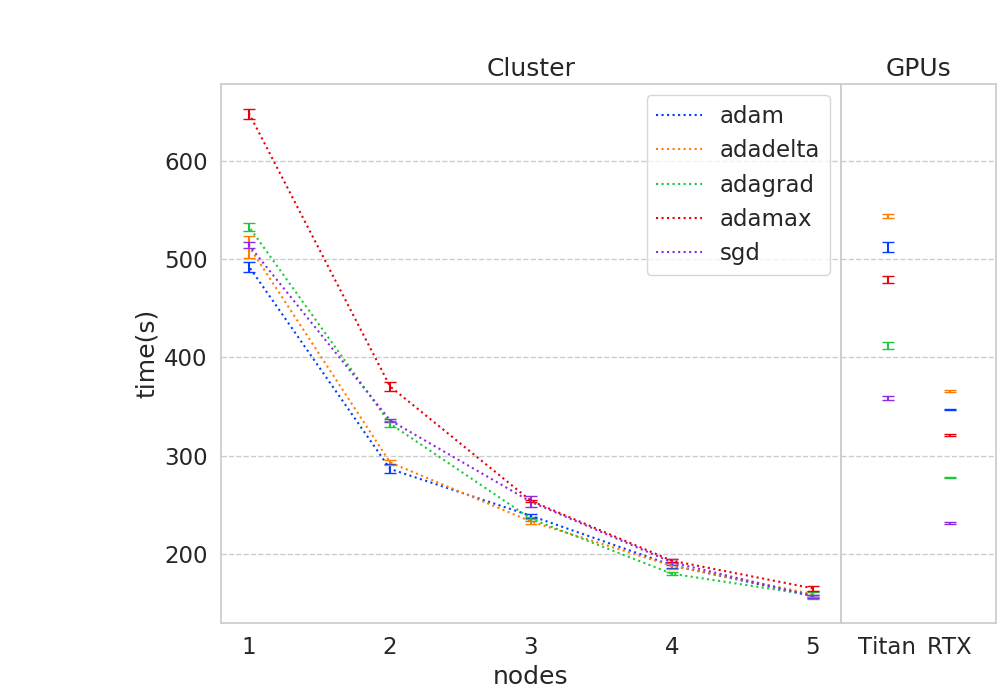
\includegraphics[scale=0.4]{figures/absolute.png}
 \caption{Number of nodes versus execution time for $1$ epoch}
 \label{1}
\end{figure}
\begin{figure}[H]
 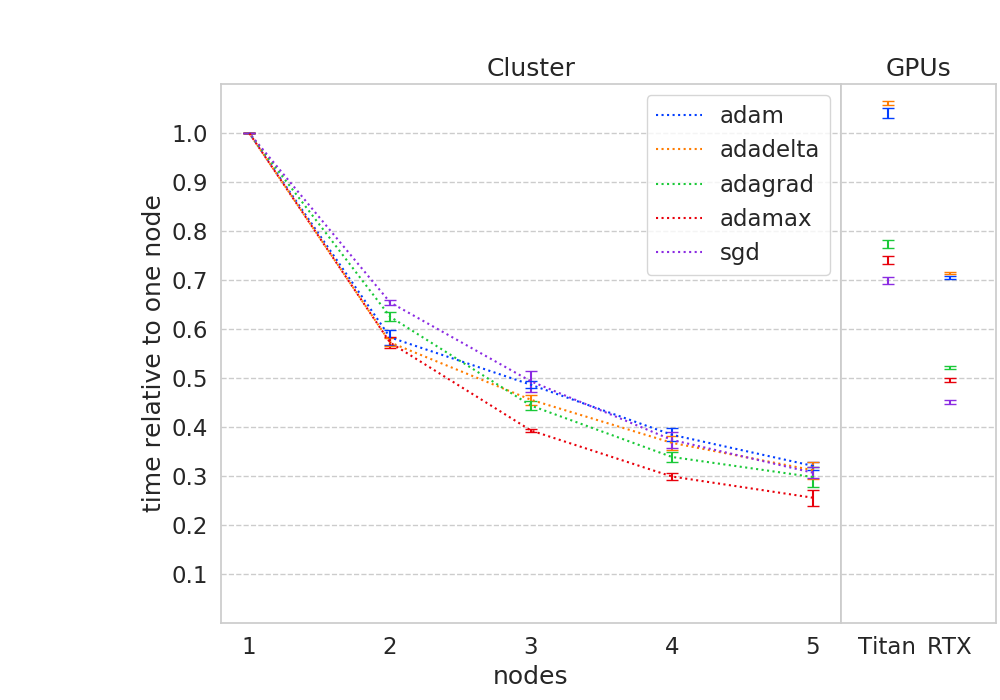
\includegraphics[scale=0.4]{figures/relative.png}
 \caption{Relative time regard execution with one node}
 \label{2}
\end{figure}

As shown in the Fig.~\ref{1} the performances improve by adding nodes, as intended. The
improvement is not linear, the difference in time performance between optimizers decrease
with increasing number of nodes. A simple interpretation could be that with more nodes
the training bottleneck is on the network side so the difference in time performance
between optimizers become less significant.
To support this hypothesis in Fig.~\ref{2} it can be seen that performance increase
approximately by $30\%$ - $40\%$ for each added node but relative improvement shrink
with the increment of the nodes. This may be due to the fact that the increase in the
number of nodes is limited by the time required for their communication with the
master.

The graphs also show that latest \textit{Nvidia} consumer-grade GPUs have comparable
performance with multi-cores CPUs.
Remembering that every node has $8$ it can be seen that in this test the \textit{Titan Xp}
can compete with an $8$ - $16$ cores cluster, depending on the chosen optimizer.
The \textit{rtx 2080} gets better results and is comparable with the performance of a $16$ -
$32$ cores cluster. This difference could be related to the different GPUs
\textit{Pascal}~\cite{pascal} and \textit{Turing}~\cite{turing} architectures. It could
be also noted that in this case the performances are strongly influenced by the chosen
optimizer. Not easily explainable this aspect should be further explored.


\chapter{Conclusion}
In this thesis work new computational paradigms have been explored. The results
with cluster architecture seems promising. They show that this technique has a
good capability to scale as the number of nodes and computational resources
increases. This characteristic can be exploit for develop large scale system.

Results with GPUs show that them can compete with cluster computing but seems
less encouraging than expected. This can be related with a number of factors such
as, for example, the kind of problem, the implementation or the hyperparameters choice.

Nevertheless, the results are promising, clustering and GPUs are definitely good
ways to improve performance of deep neural networks for solve a discrimination signal background problem.

% Backmatter
\appendix
\cleardoublepage\defbibheading{bibintoc}[\bibname]{%
 \phantomsection
 \manualmark
 \markboth{\spacedlowsmallcaps{#1}}{\spacedlowsmallcaps{#1}}%
 \addtocontents{toc}{\protect\vspace{\beforebibskip}}%
 \addcontentsline{toc}{chapter}{\tocEntry{#1}}%
 \chapter*{#1}%
}

\printbibliography[heading=bibintoc]

\end{document}
